%%%%%%%%%%%%%%%%%%%%%%%%%%%%%%%%%%%%%%%%%
%----------------------------------------------------------------------------------------
%	PACKAGES AND OTHER DOCUMENT CONFIGURATIONS
%----------------------------------------------------------------------------------------

\documentclass[12pt]{article}

\usepackage{amsmath}

\usepackage{graphicx}

\usepackage{hyperref}

\usepackage[utf8]{inputenc}

%%%%%%%%%%%%%%%%%%%%%%%%%%%%%%%%%%%%%%%%%
% Arsclassica Article
% Structure Specification File
%
% This file has been downloaded from:
% http://www.LaTeXTemplates.com
%
% Original author:
% Lorenzo Pantieri (http://www.lorenzopantieri.net) with extensive modifications by:
% Vel (vel@latextemplates.com)
%
% License:
% CC BY-NC-SA 3.0 (http://creativecommons.org/licenses/by-nc-sa/3.0/)
%
%%%%%%%%%%%%%%%%%%%%%%%%%%%%%%%%%%%%%%%%%

%----------------------------------------------------------------------------------------
%	REQUIRED PACKAGES
%----------------------------------------------------------------------------------------

\usepackage[
nochapters, % Turn off chapters since this is an article        
beramono, % Use the Bera Mono font for monospaced text (\texttt)
eulermath,% Use the Euler font for mathematics
pdfspacing, % Makes use of pdftex’ letter spacing capabilities via the microtype package
dottedtoc % Dotted lines leading to the page numbers in the table of contents
]{classicthesis} % The layout is based on the Classic Thesis style

\usepackage{arsclassica} % Modifies the Classic Thesis package

\usepackage[T1]{fontenc} % Use 8-bit encoding that has 256 glyphs

\usepackage[utf8]{inputenc} % Required for including letters with accents

\usepackage{graphicx} % Required for including images
\graphicspath{{Figures/}} % Set the default folder for images

\usepackage{enumitem} % Required for manipulating the whitespace between and within lists

\usepackage{lipsum} % Used for inserting dummy 'Lorem ipsum' text into the template

\usepackage{subfig} % Required for creating figures with multiple parts (subfigures)

\usepackage{amsmath,amssymb,amsthm} % For including math equations, theorems, symbols, etc

\usepackage{varioref} % More descriptive referencing

\usepackage{makeidx}
%----------------------------------------------------------------------------------------
%	THEOREM STYLES
%---------------------------------------------------------------------------------------

\theoremstyle{definition} % Define theorem styles here based on the definition style (used for definitions and examples)
\newtheorem{definition}{Definition}

\theoremstyle{plain} % Define theorem styles here based on the plain style (used for theorems, lemmas, propositions)
\newtheorem{theorem}{Theorem}

\theoremstyle{remark} % Define theorem styles here based on the remark style (used for remarks and notes)

%----------------------------------------------------------------------------------------
%	HYPERLINKS
%---------------------------------------------------------------------------------------

\hypersetup{
%draft, % Uncomment to remove all links (useful for printing in black and white)
colorlinks=true, breaklinks=true, bookmarks=true,bookmarksnumbered,
urlcolor=webbrown, linkcolor=RoyalBlue, citecolor=webgreen, % Link colors
pdftitle={Darkly: There is something wrong...}, % PDF title
pdfauthor={Sibonelo Nkosi \textcopyright}, % PDF Author
pdfsubject={Web Security}, % PDF Subject
pdfkeywords={WeThinkCode}, % PDF Keywords
pdfcreator={pdfLaTeX}, % PDF Creator
pdfproducer={LaTeX with hyperref and ClassicThesis} % PDF producer
} % Include the structure.tex file which specified the document structure and layout

\hyphenation{Fortran hy-phen-ation} % Specify custom hyphenation points in words with dashes where you would like hyphenation to occur, or alternatively, don't put any dashes in a word to stop hyphenation altogether
%----------------------------------------------------------------------------------------
%	CODE SNIPPET INSERTION
\usepackage{listings} % Required for inserting code snippets
%\usepackage[usenames,dvipsnames]{color} % Required for specifying custom colors and referring to colors by name

\definecolor{DarkGreen}{rgb}{0.0,0.4,0.0} % Comment color
\definecolor{highlight}{RGB}{255,251,204} % Code highlight color

\lstdefinestyle{Style1}{ % Define a style for your code snippet, multiple definitions can be made if, for example, you wish to insert multiple code snippets using different programming languages into one document
language=Perl, % Detects keywords, comments, strings, functions, etc for the language specified
backgroundcolor=\color{highlight}, % Set the background color for the snippet - useful for highlighting
basicstyle=\footnotesize\ttfamily, % The default font size and style of the code
breakatwhitespace=false, % If true, only allows line breaks at white space
breaklines=true, % Automatic line breaking (prevents code from protruding outside the box)
captionpos=b, % Sets the caption position: b for bottom; t for top
commentstyle=\usefont{T1}{pcr}{m}{sl}\color{DarkGreen}, % Style of comments within the code - dark green courier font
deletekeywords={}, % If you want to delete any keywords from the current language separate them by commas
%escapeinside={\%}, % This allows you to escape to LaTeX using the character in the bracket
firstnumber=1, % Line numbers begin at line 1
frame=single, % Frame around the code box, value can be: none, leftline, topline, bottomline, lines, single, shadowbox
frameround=tttt, % Rounds the corners of the frame for the top left, top right, bottom left and bottom right positions
keywordstyle=\color{Blue}\bf, % Functions are bold and blue
morekeywords={}, % Add any functions no included by default here separated by commas
numbers=left, % Location of line numbers, can take the values of: none, left, right
numbersep=10pt, % Distance of line numbers from the code box
numberstyle=\tiny\color{Gray}, % Style used for line numbers
rulecolor=\color{black}, % Frame border color
showstringspaces=false, % Don't put marks in string spaces
showtabs=false, % Display tabs in the code as lines
stepnumber=5, % The step distance between line numbers, i.e. how often will lines be numbered
stringstyle=\color{Purple}, % Strings are purple
tabsize=2, % Number of spaces per tab in the code
}

% Create a command to cleanly insert a snippet with the style above anywhere in the document
\newcommand{\insertcode}[2]{\begin{itemize}\item[]\lstinputlisting[caption=#2,label=#1,style=Style1]{#1}\end{itemize}} % The first argument is the script location/filename and the second is a caption for the listing
%----------------------------------------------------------------------------------------

\makeindex
\begin{document}

%----------------------------------------------------------------------------------------
%	HEADERS
%----------------------------------------------------------------------------------------

\renewcommand{\sectionmark}[1]{\markright{\spacedlowsmallcaps{#1}}} % The header for all pages (oneside) or for even pages (twoside)
%\renewcommand{\subsectionmark}[1]{\markright{\thesubsection~#1}} % Uncomment when using the twoside option - this modifies the header on odd pages
\lehead{\mbox{\llap{\small\thepage\kern1em\color{halfgray} \vline}\color{halfgray}\hspace{0.5em}\rightmark\hfil}} % The header style

\pagestyle{scrheadings} % Enable the headers specified in this block

%%%%%%%%%%%%%%%%%%%%%%%%%%%%%%%%%%%%%%%%%
% Academic Title Page
% LaTeX Template
% Version 2.0 (17/7/17)
%
% 
%
%%%%%%%%%%%%%%%%%%%%%%%%%%%%%%%%%%%%%%%%%

%----------------------------------------------------------------------------------------
%	PACKAGES AND OTHER DOCUMENT CONFIGURATIONS
%----------------------------------------------------------------------------------------

%\documentclass[11pt]{article}

%\usepackage[utf8]{inputenc} % Required for inputting international characters
%\usepackage[T1]{fontenc} % Output font encoding for international characters

%\usepackage{mathpazo} % Palatino font

%\begin{document}

%----------------------------------------------------------------------------------------
%	TITLE PAGE
%----------------------------------------------------------------------------------------

\begin{titlepage} % Suppresses displaying the page number on the title page and the subsequent page counts as page 1
	\newcommand{\HRule}{\rule{\linewidth}{0.5mm}} % Defines a new command for horizontal lines, change thickness here
	
	\center % Centre everything on the page
	
	%------------------------------------------------
	%	Headings
	%------------------------------------------------
	
	\textsc{\LARGE WeThinkCode\_}\\[1.5cm] % Main heading such as the name of your university/college
	
	\textsc{\Large WEB II}\\[0.5cm] % Major heading such as course name
	
	\textsc{\large Project II}\\[0.5cm] % Minor heading such as course title
	
	%------------------------------------------------
	%	Title
	%------------------------------------------------
	
	\HRule\\[0.4cm]
	
	{\huge\bfseries Darkly: }\\{\large There is something wrong...}\\[0.4cm] % Title of your document
	
	\HRule\\[1.5cm]
	
	%------------------------------------------------
	%	Author(s)
	%------------------------------------------------
	
	% \begin{minipage}{0.4\textwidth}
	% 	\begin{flushleft}
	% 		\large
	% 		\textit{Developer}\\
	% 		Mosima \textsc{Mamaleka} % Your name
	% 	\end{flushleft}
	% \end{minipage}
	% ~
	% \begin{minipage}{0.4\textwidth}
	% 	\begin{flushright}
	% 		\large
	% 		\textit{Developer}\\
	% 		Sibonelo \textsc{Nkosi} % Supervisor's name
	% 	\end{flushright}
	% \end{minipage}
	
	% If you don't want a supervisor, uncomment the two lines below and comment the code above
	{\large\textit{Developer}}\\
	Sibonelo \textsc{Nkosi}\\ % Your name
	Username: \textsc{sinkosi} % Your name

	\vfill
	{\large\textit{Assessor}}\\
	Mufaro \textsc{Simbisayi}\\ % Your name
	%------------------------------------------------
	%	Date
	%------------------------------------------------
	
	\vfill\vfill\vfill % Position the date 3/4 down the remaining page
	
	\large{October 2020}\\ % Date, change the \today to a set date if you want to be precise
	
	%------------------------------------------------
	%	Logo
	%------------------------------------------------
	
	\vfill\vfill
	
	
\includegraphics[width=0.2\textwidth]{0.title/index.png}\\[1cm] % Include a department/university logo - this will require the graphicx package
	
\includegraphics[width=0.2\textwidth]{0.title/docker.png}\\[1cm] % Include a department/university logo - this will require the graphicx package
	%----------------------------------------------------------------------------------------
	
	\vfill % Push the date up 1/4 of the remaining page
	
\end{titlepage}

%----------------------------------------------------------------------------------------

%\end{document}


%----------------------------------------------------------------------------------------
%	TABLE OF CONTENTS & LISTS OF FIGURES AND TABLES
%----------------------------------------------------------------------------------------
\newpage
%\maketitle % Print the title/author/date block

\setcounter{tocdepth}{3} % Set the depth of the table of contents to show sections and subsections only

\tableofcontents % Print the table of contents

\newpage

%\listoffigures % Print the list of figures

%\listoftables % Print the list of tables


%----------------------------------------------------------------------------------------
%	ABSTRACT
%----------------------------------------------------------------------------------------

\newpage

\section{Introduction}

The aim of this project is to introduce you to computer security in the web domain.
You will be able to discover OWASP, which is, no more and no less, the biggest web
security project to date.
You will also understand what a lot of frameworks do in an automatic and completely
transparent way for you.

You will need to use a virtual machine 
(i386) to validate this project. Once your
machine is started with the ISO supplied with the subject.
Requirements:
\begin{itemize}
    \item Virtual Box
    \item darkly.iso (\href{https://drive.google.com/file/d/145dbZHjZWyMiRscj-72jE3n5PM5vXyB9/view?usp=sharing}{download here} )
    \item Patience
    \item The Ability to keep your wits about you
    \item Other stuff (probably)
\end{itemize}

%Summary of the stuff

\begin{table}[hbt]
    \caption{Table of Grades}
    \centering
    \begin{tabular}{llr}
    \toprule
    \multicolumn{2}{c}{Name} \\
    \cmidrule(r){1-2}
    First name & Last Name & Grade \\
    \midrule
    John & Doe & $7.5$ \\
    Richard & Miles & $2$ \\
    \bottomrule
    \end{tabular}
    \label{tab:label}
    \end{table}
    
    Reference to Table~\vref{tab:label}. % The \vref command specifies the location of the reference
    
    

\section{Getting Started}

\subsection{Windows}

Windows Installation\textsuperscript{*}: Ensure that you have the latest version
of VirtualBox for Windows or download it from the \href{http://www.google.com}{VirtualBox Website} or
Windows Store.

\let\thefootnote\relax\footnotetext{\textsuperscript{*} \textit{Information provided is correct for current users configuration i.e Windows Home 10:2004, results
may differ for other configurations }}

%---------------------
\subsubsection{Create Virtual Machine}
\begin{figure}[!htb]
    \centering
    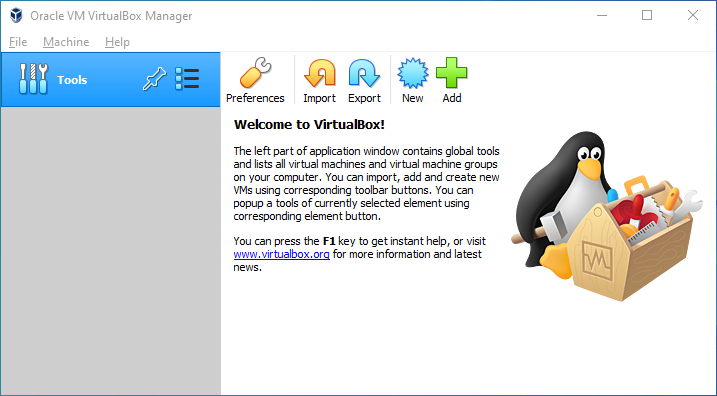
\includegraphics[width=0.752\textwidth]{images/Win00-00.png}\\[0cm]  
    \caption[Windows Virtual Box]{New Virtual Machine Setup}
    \label{fig:00-01 - Windows Virtual Box New VM} 
\end{figure}
Begin by Creating a new Virtual Machine. To do this click on the blue icon
labelled new as shown in Figure \vref{fig:00-01 - Windows Virtual Box New VM}.

%---------------------
\subsubsection{Name \& Operating System}
\begin{figure}[!htb]
    \centering
    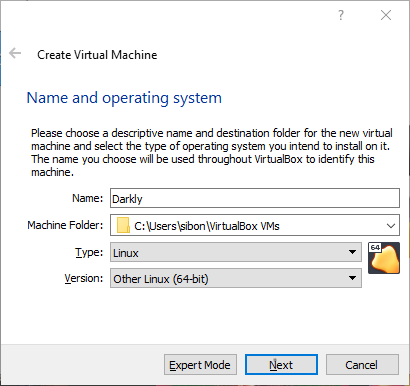
\includegraphics[width=0.752\textwidth]{images/Win00-01.png}\\[0cm]  
    \caption[Windows Virtual Box]{Setup Of Operating System Type and Name}
    \label{fig:00-02 - Windows Virtual Box Operating System} 
\end{figure}
You have to give your Virtual Machine a new name, I have chosen 'Darkly'. Make
sure to pick a folder for storage of the Virtual Machine or leave it to the
default provided by Virtual Box.

You will have to choose the 'type' of machine you are creating. At this point
you must select 'Linux' as this is what the Darkly.iso is based from. You will
be given options or 'flavours' to choose from. Pick 'Other 64-bit'. This is
best shown in Figure ~\Vref{fig:00-02 - Windows Virtual Box Operating System}.

Please do take note that the Darkly VM will not work if it is not 64-bit.

%---------------------
\subsubsection{Memory Size}
\begin{figure}[!htb]
    \centering
    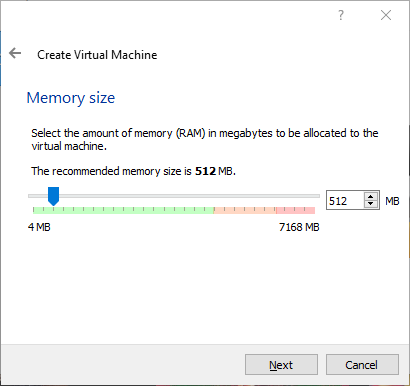
\includegraphics[width=0.752\textwidth]{images/Win00-02.png}\\[0cm]  
    \caption[Windows Virtual Box]{Virtual Box Memory Size Settings}
    \label{fig:00-03 - Windows Virtual Box Memory Size} 
\end{figure}
Selecting a memory size is the next step. Darkly will not be actively running
as another Virtual Machine would. Therefore only a limited amount of RAM is
required. The recommended size is 512MB.

To set the memory size, a slide is used, as shown in Figure \Vref{fig:00-03 - Windows Virtual Box Memory Size}.

You can also set it using manually by typing in the value.

%---------------------
\subsubsection{Hard Disk File Type}
\begin{figure}[!htb]
    \centering
    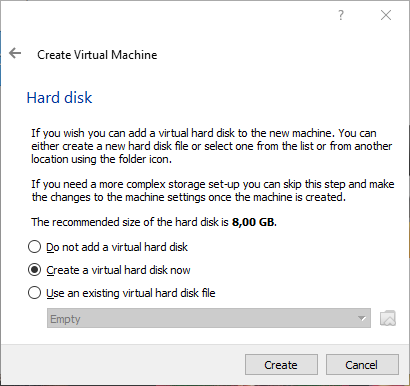
\includegraphics[width=0.752\textwidth]{images/Win00-03.png}\\[0cm]  
    \caption[Windows Virtual Box]{Virtual Box Disk Type}
    \label{fig:00-04 - Windows Virtual Box Disk Type} 
\end{figure}
Select VirtualBox Disk Image as shown in Figure \Vref{fig:00-04 - Windows Virtual Box Disk Type}.
This is the best decision because the Machine will not be migrated to other
Virtual Machine Players like VMWare etc. The use is short-term.

%---------------------
\subsubsection{Storage Type}
\begin{figure}[!htb]
    \centering
    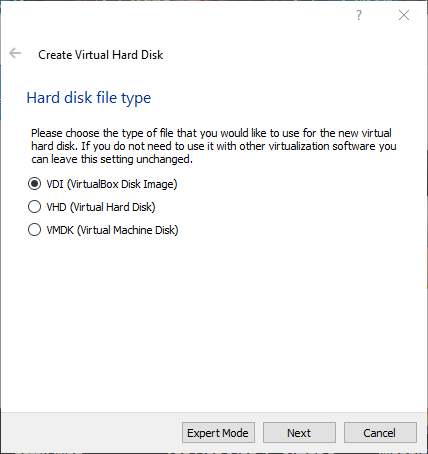
\includegraphics[width=0.752\textwidth]{images/Win00-04.png}\\[0cm]  
    \caption[Windows Virtual Box]{Virtual Box Storage Type}
    \label{fig:00-05 - Windows Virtual Box Storage Type} 
\end{figure}
Ensure that you have the size Dynamically allocated as shown in Figure \Vref{fig:00-05 - Windows Virtual Box Storage Type}.
If you would like a fixed size, it is okay, but this entails your Hard Disk
being allocated upfront.

Please note, you have not selected your Hard Disk size so it is key to ensure
you are aware of how much space you have free before allocating a fixed space size.

%---------------------
\subsubsection{File Location \& Size}
\begin{figure}[!htb]
    \centering
    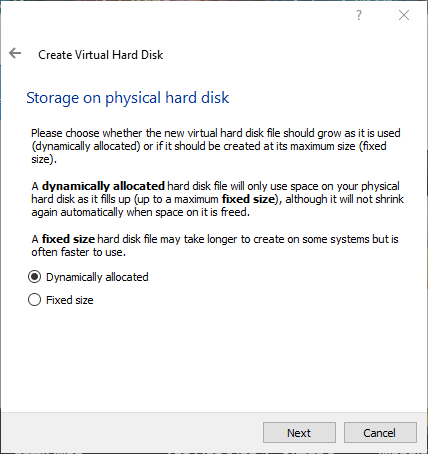
\includegraphics[width=0.752\textwidth]{images/Win00-05.png}\\[0cm]  
    \caption[Windows Virtual Box]{Virtual Box Hard Disk Location and Size}
    \label{fig:00-06 - Windows Virtual Box Hard Disk} 
\end{figure}
This is where you can set up the location for your Virtual Box Machine to
store its data. Remember that the machine can be stored in one location but
the simulation of its Hard Disk can be stored on a Flash Drive or External
Drive if you wish.\\

I have decided to retain the local drive as the storage location. This is 
the default VirtualBox directory. You can select any size you wish, I have
selected 1,99GB to keep my box small as shown in Figure \Vref{fig:00-06 - Windows Virtual Box Hard Disk}.
I can ammend this later if I need to.

%---------------------
\subsubsection{Mount Disk Image}
\begin{figure}[!htb]
    \centering
    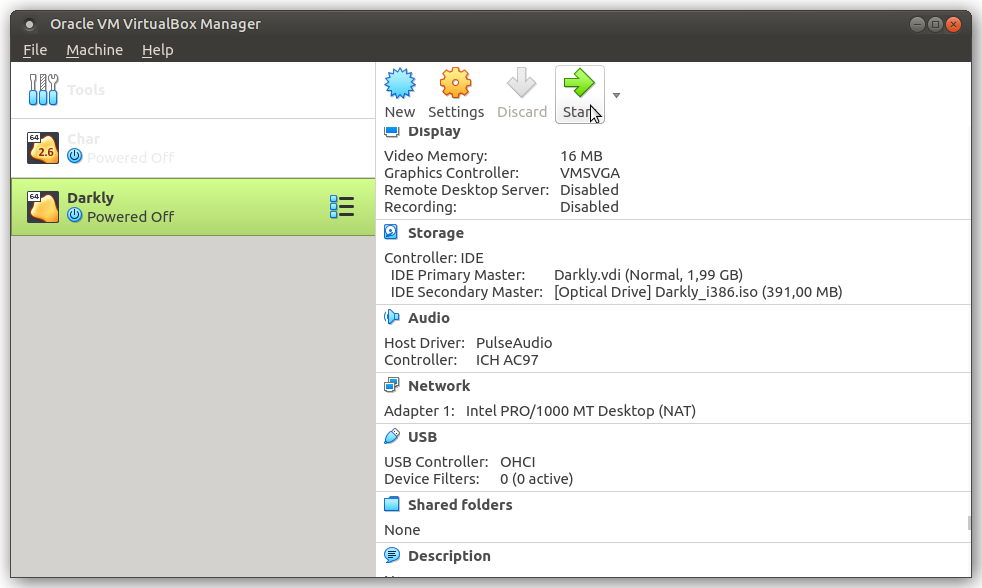
\includegraphics[width=0.752\textwidth]{images/00-07.png}\\[0cm]  
    \caption[Windows Virtual Box]{Virtual Box Setup of Disk Drive Mount Darkly.iso Image}
    \label{fig:00-07 - Windows Virtual Box ISO Mount} 
\end{figure}
The next step is to mount the Darkly.iso disk as a form of storage. Click on
your image 'Darkly' or whatever you may have named it, on the lefthand navigation
panel as shown in Figure \Vref{fig:00-07 - Windows Virtual Box ISO Mount}.\\

Next click on Settings -> Storage -> IDE Secondary Master. After this, navigate
to the folder where the ISO is located. Mount it and you will see it listed
as shown in Figure \Vref{fig:00-07 - Windows Virtual Box ISO Mount}.\\

Click Start (Green arrow pointing right) to commence running the image.

%---------------------
\subsubsection{Run Disk Image}
\begin{figure}[!htb]
    \centering
    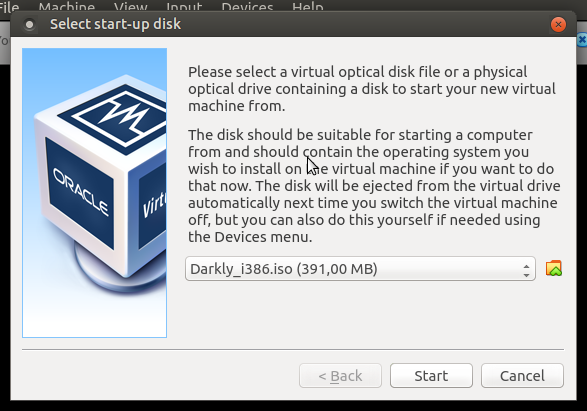
\includegraphics[width=0.752\textwidth]{images/00-08.png}\\[0cm]  
    \caption[Windows Virtual Box]{Virtual Box Start-up Disk Selector}
    \label{fig:00-08 - Windows Virtual Box Startup Disk Selector} 
\end{figure}
As shown in Figure ~\vref{fig:00-08 - Windows Virtual Box Startup Disk Selector},
you are expected to select 'Darkly\_i386.iso' as the start-up disk. This will
then complete the Installation process.

%---------------------
\subsubsection{Running but Incomplete}
\begin{figure}[!htb]
    \centering
    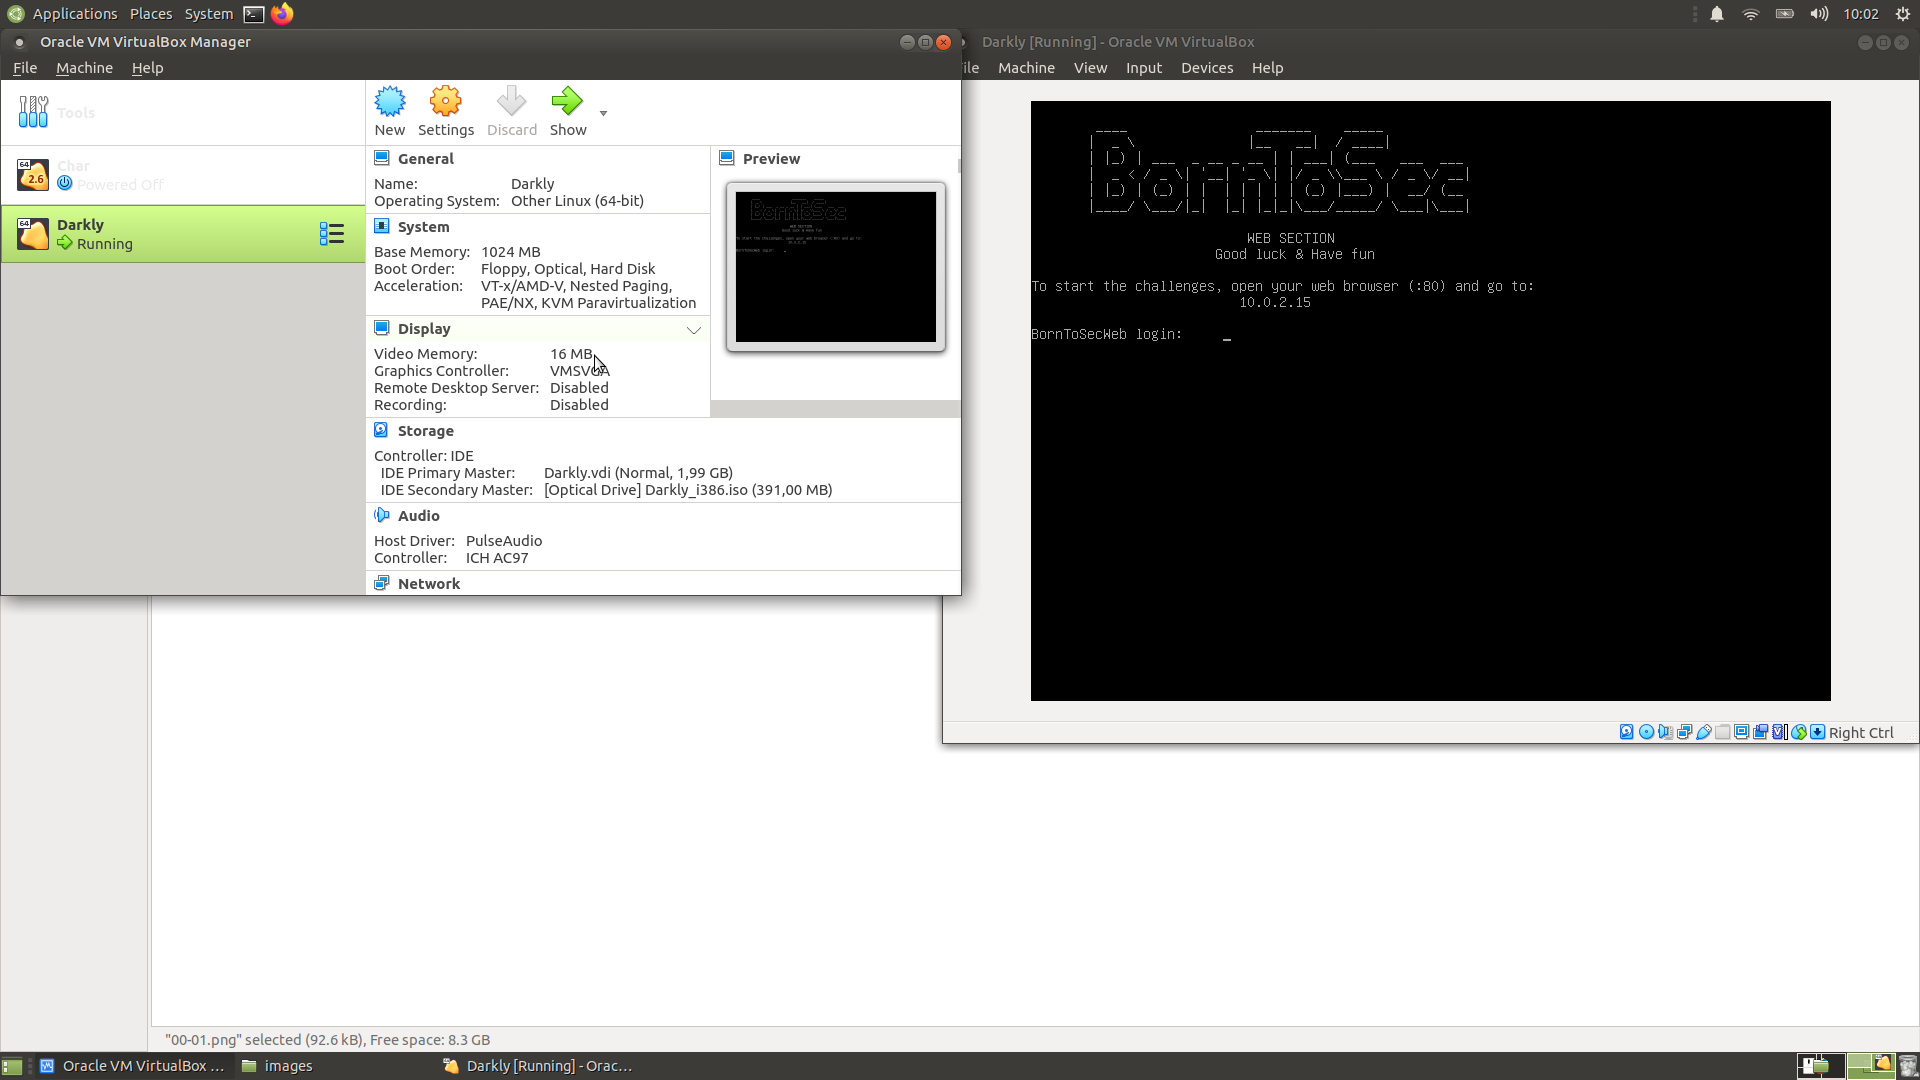
\includegraphics[width=0.752\textwidth]{images/00-09.png}\\[0cm]  
    \caption[Windows Virtual Box]{\emph{Virtual Box Landing}, on Ubuntu}
    \label{fig:00-09 - Windows Virtual Box Running not complete} 
\end{figure}
You have successfully installed the VM and it is running. The IP address is
printed on the screen. ...I bet that the IP address does not really work\dots\\

This needs you to go to settings as shown in Figure \vref{fig:00-10 - Windows Virtual Box Set Bridge}

%---------------------
\subsubsection{Set Network Bridge}

\begin{figure}[!htb]
    \centering
    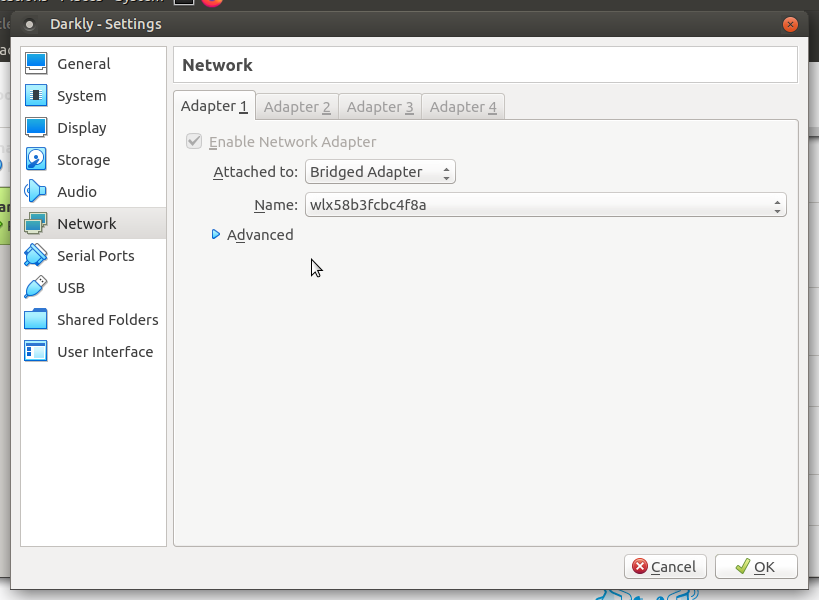
\includegraphics[width=0.752\textwidth]{images/00-10.png}\\[0cm]  
    \caption[Windows Virtual Box]{\emph{Virtual Box Landing}, on Ubuntu}
    \label{fig:00-10 - Windows Virtual Box Set Bridge} 
\end{figure}
On the lefthand navigation-bar, Select Network -> Adaptor 1.
Change the settings from a NAT Adaptor as would be the default, and set it
to a 'Bridge' connection. as shown in Figure \vref{fig:00-10 - Windows Virtual Box Set Bridge}.

%---------------------
\subsubsection{Don't Panic! Loading Screen}

\begin{figure}[!htb]
    \centering
    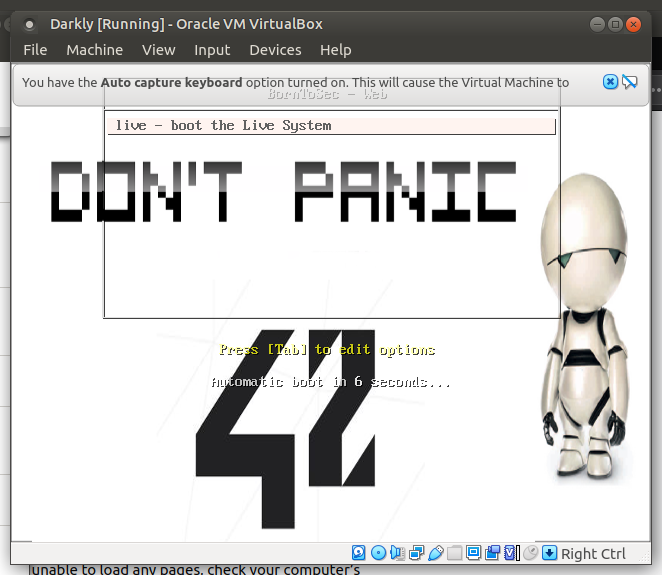
\includegraphics[width=0.752\textwidth]{images/00-11.png}\\[0cm]  
    \caption[Windows Virtual Box]{Virtual Box Loading Screen Splash with Hitchhiker's Guide Robot}
    \label{fig:00-11 - Windows Virtual Box LoadingScreen1} 
\end{figure}
\subparagraph{Don't Panic, it's just a loading screen}

%---------------------
\subsubsection{More Loading Screens}
\begin{figure}[!htb]
    \centering
    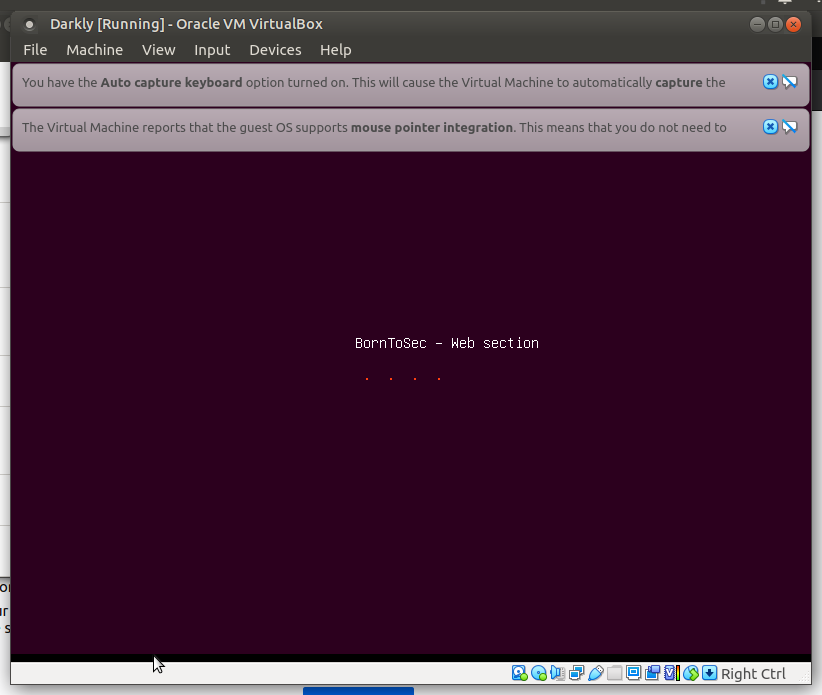
\includegraphics[width=0.752\textwidth]{images/00-12.png}\\[0cm]  
    \caption[Windows Virtual Box]{More Virtual Box Loading Screens}
    \label{fig:00-12 - Windows Virtual Box LoadingScreen2} 
\end{figure}
If you are seeing the figure shown in Figure \vref{fig:00-12 - Windows Virtual Box LoadingScreen2}
you are making good progress and must hang in there.

%---------------------
\subsubsection{Up \& Running}

\begin{figure}[!htb]
    \centering
    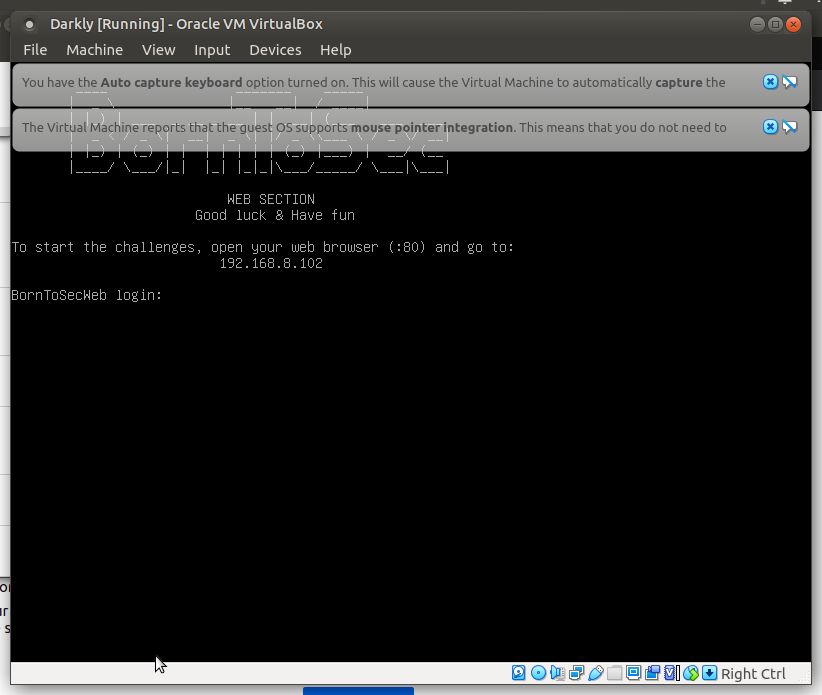
\includegraphics[width=0.752\textwidth]{images/00-13.png}\\[0cm]  
    \caption[Windows Virtual Box]{Virtual Box Fully Loaded Screen with IP Address \& Prompt}
    \label{fig:00-13 - Windows Virtual Box LoadedIP} 

\end{figure}
The new IP Address should look different to the first one and should be similar to
your own IP address after runnung 'ifconfig'.
You should see a similar figure to that shown in Figure \vref{fig:00-13 - Windows Virtual Box LoadedIP}.

%---------------------
\subsubsection{BornToSec}
\begin{figure}[!htb]
    \centering
    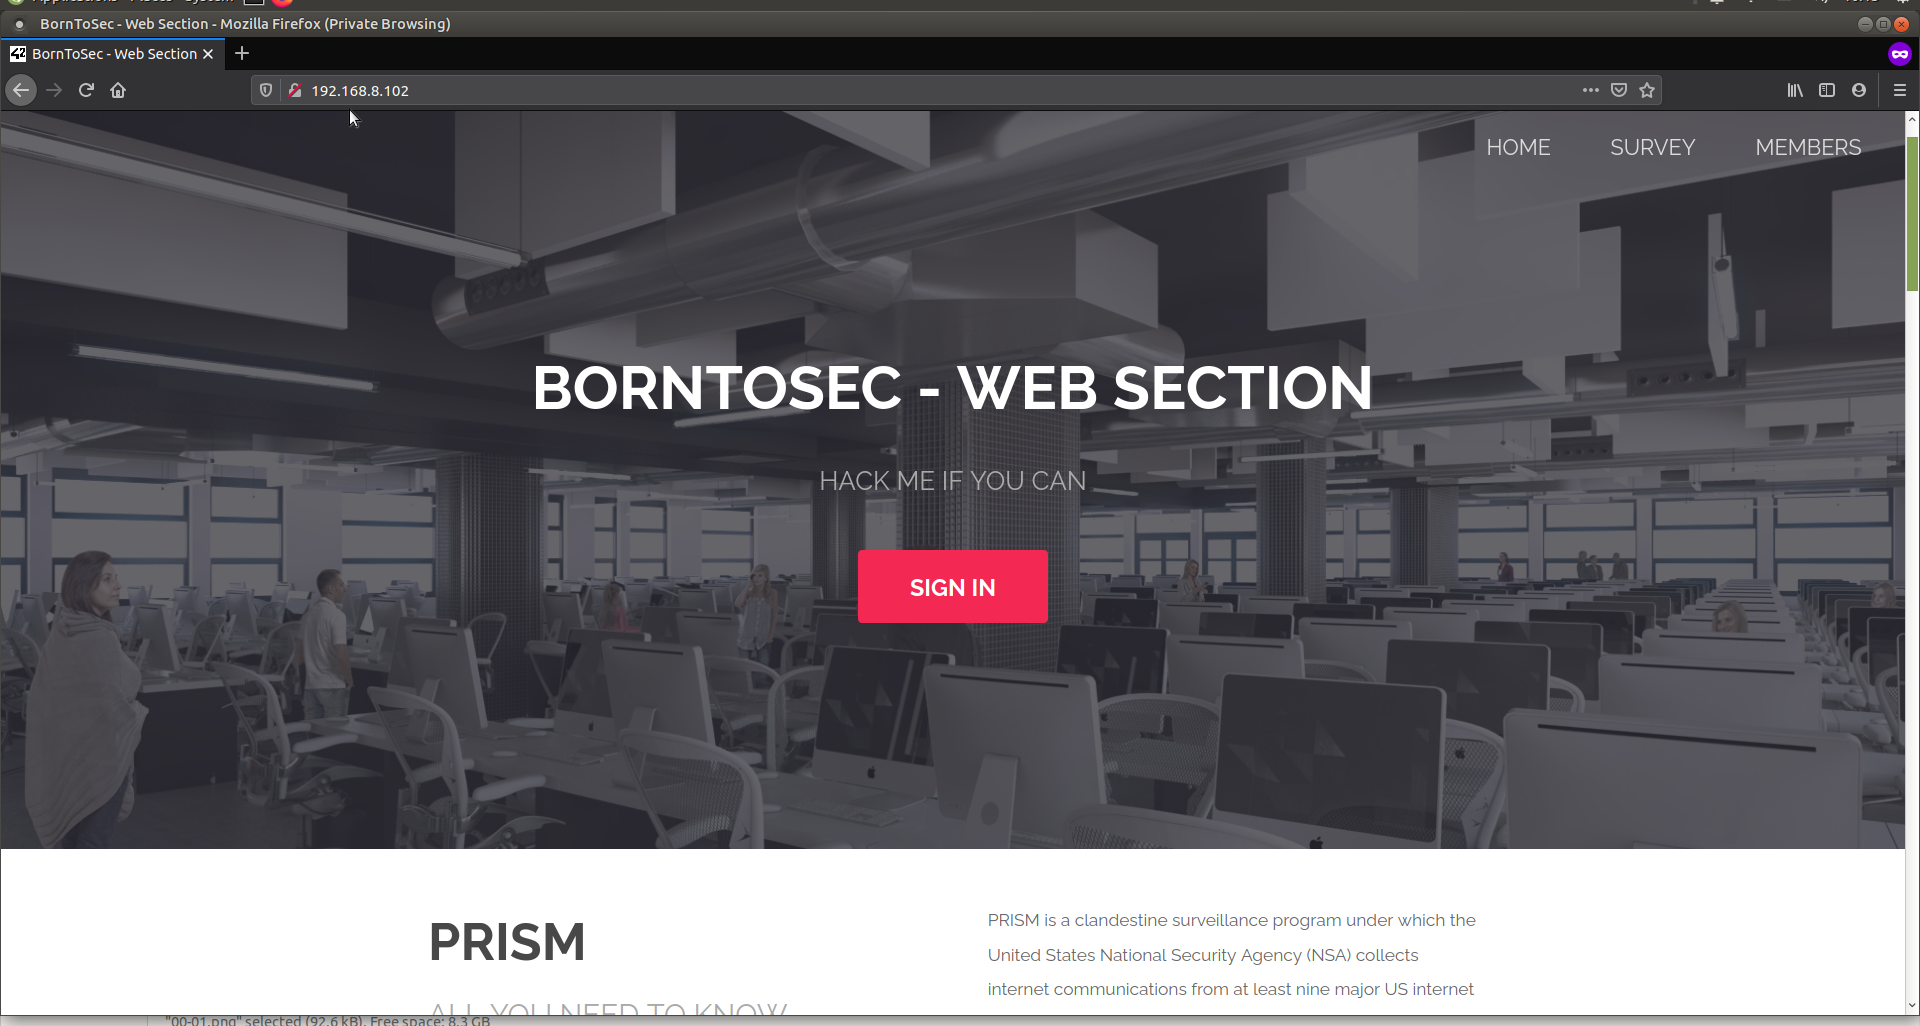
\includegraphics[width=0.752\textwidth]{images/00-14.png}\\[0cm]  
    \caption[Windows Virtual Box]{BornToSec Homepage}
    \label{fig:00-14 - Windows Virtual Box HomePage} 
\end{figure}
If you see the same figure on your screen as the one shown on Figure \vref{fig:00-14 - Windows Virtual Box HomePage},
then you have successfully setup your Virtual Machine.

\paragraph{Time To DO The FUN Stuff!}

%----------------------------------------------------------------------------------------
%	Footnotes
%----------------------------------------------------------------------------------------

%\let\thefootnote\relax\footnotetext{\textsuperscript{*} \textit{Information provided is correct for current users configuration i.e Windows Home 10:2004, results
%may differ for other configurations }}

%----------------------------------------------------------------------------------------

\subsection{Linux}

\noindent Linux Installation\textsuperscript{**}: Begin by ensuring that you have Virtual Box installed on your system, if not type:
\begin{lstlisting}[language=bash]
    $ sudo apt-get install virtualbox
\end{lstlisting}
%\vfill
\let\thefootnote\relax\footnotetext{\textsuperscript{**} \textit{Snap install is not available for all Linux Distros, this is expected to work on Ubuntu and Debian flavours}}
%---------------------
\subsubsection{Create Virtual Machine}
\begin{figure}[!htb]
    \centering
    %\insertcode{Scripts/example.pl}{Nena would be proud.} % The first argument is the script location/filename and the second is a caption for the listing
    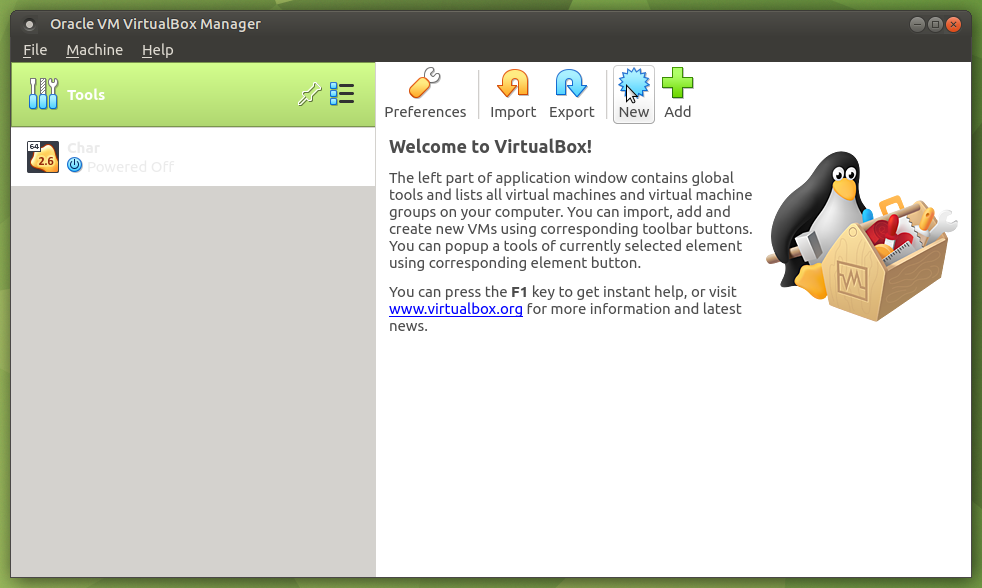
\includegraphics[width=0.752\textwidth]{images/00-0.png}\\[0cm]  
    \caption[Virtual Box]{New Virtual Machine Setup}
    %from \url{http://localhost:3000/}).} % The text in the square bracket is the caption for the list of figures while the text in the curly brackets is the figure caption
    \label{fig:00-01 - Linux Virtual Box New VM} 
\end{figure}
Begin by Creating a new Virtual Machine. To do this click on the blue icon
labelled new as shown in Figure \vref{fig:00-01 - Linux Virtual Box New VM}.

%---------------------
\subsubsection{Name \& Operating System}
\begin{figure}[!htb]
    \centering
    %\insertcode{Scripts/example.pl}{Nena would be proud.} % The first argument is the script location/filename and the second is a caption for the listing
    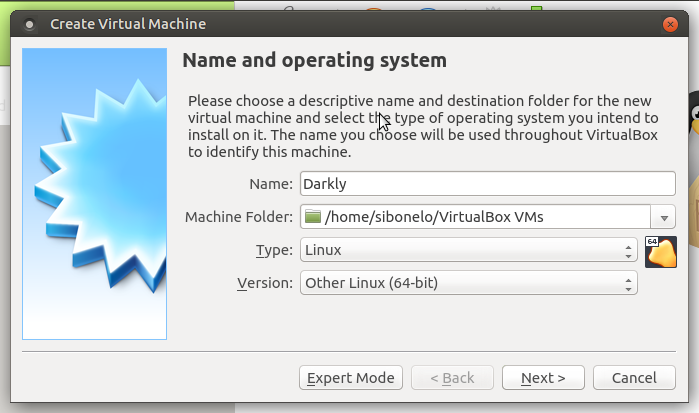
\includegraphics[width=0.752\textwidth]{images/00-01.png}\\[0cm]  
    \caption[Virtual Box]{Setup Of Operating System Type and Name}
    \label{fig:00-02 - Linux Virtual Box Operating System} 
\end{figure}
You have to give your Virtual Machine a new name, I have chosen 'Darkly'. Make
sure to pick a folder for storage of the Virtual Machine or leave it to the
default provided by Virtual Box.

You will have to choose the 'type' of machine you are creating. At this point
you must select 'Linux' as this is what the Darkly.iso is based from. You will
be given options or 'flavours' to choose from. Pick 'Other 64-bit'. This is
best shown in Figure ~\Vref{fig:00-02 - Linux Virtual Box Operating System}.

Please do take note that the Darkly VM will not work if it is not 64-bit.

%---------------------
\subsubsection{Memory Size}
\begin{figure}[!htb]
    \centering
    %\insertcode{Scripts/example.pl}{Nena would be proud.} % The first argument is the script location/filename and the second is a caption for the listing
    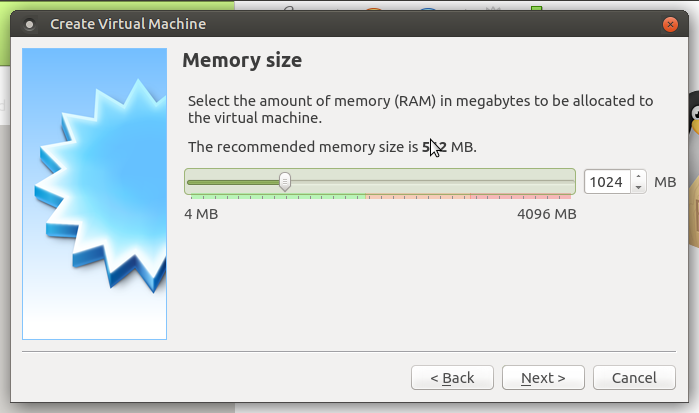
\includegraphics[width=0.752\textwidth]{images/00-02.png}\\[0cm]  
    \caption[Virtual Box]{Virtual Box Memory Size Settings}
    %from \url{http://localhost:3000/}).} % The text in the square bracket is the caption for the list of figures while the text in the curly brackets is the figure caption
    \label{fig:00-03 - Linux Virtual Box Memory Size} 
\end{figure}
Selecting a memory size is the next step. Darkly will not be actively running
as another Virtual Machine would. Therefore only a limited amount of RAM is
required. The recommended size is 512MB but in my opinion I believe 1024MB is
the best.

To set the memory size, a slide is used, as shown in Figure \Vref{fig:00-03 - Linux Virtual Box Memory Size}.

You can also set it using manually by typing in the value.

%---------------------
\subsubsection{Hard Disk File Type}
\begin{figure}[!htb]
    \centering
    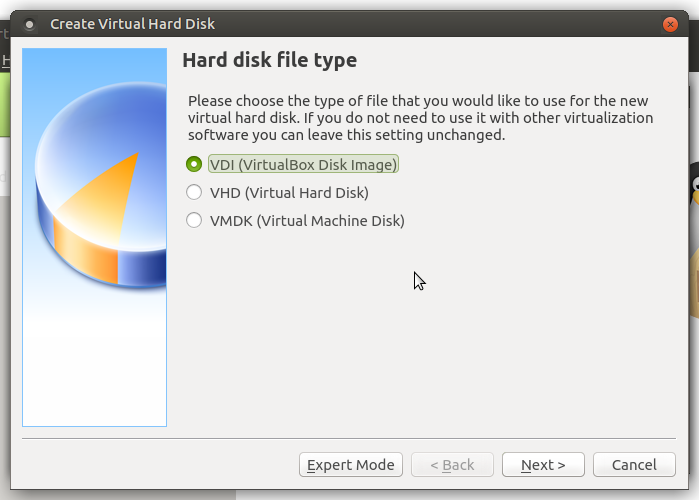
\includegraphics[width=0.752\textwidth]{images/00-03.png}\\[0cm]  
    \caption[Virtual Box]{Virtual Box Disk Type}
    \label{fig:00-04 - Linux Virtual Box Disk Type} 
\end{figure}
Select VirtualBox Disk Image as shown in Figure \Vref{fig:00-04 - Linux Virtual Box Disk Type}.
This is the best decision because the Machine will not be migrated to other
Virtual Machine Players like VMWare etc. The use is short-term.

%---------------------
\subsubsection{Storage Type}
\begin{figure}[!htb]
    \centering
    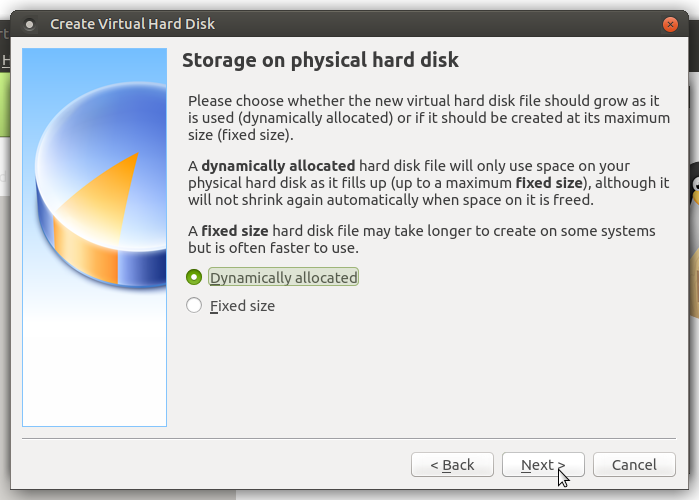
\includegraphics[width=0.752\textwidth]{images/00-04.png}\\[0cm]  
    \caption[Virtual Box]{Virtual Box Storage Type}
    \label{fig:00-05 - Linux Virtual Box Storage Type} 
\end{figure}
Ensure that you have the size Dynamically allocated as shown in Figure \Vref{fig:00-05 - Linux Virtual Box Storage Type}.
If you would like a fixed size, it is okay, but this entails your Hard Disk
being allocated upfront.

Please note, you have not selected your Hard Disk size so it is key to ensure
you are aware of how much space you have free before allocating a fixed space size.

%---------------------
\subsubsection{File Location \& Size}
\begin{figure}[!htb]
    \centering
    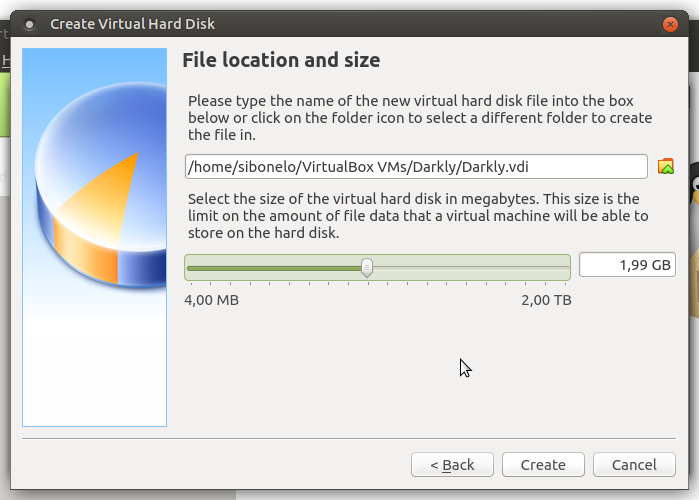
\includegraphics[width=0.752\textwidth]{images/00-05.png}\\[0cm]  
    \caption[Virtual Box]{Virtual Box Hard Disk Location and Size}
    \label{fig:00-06 - Linux Virtual Box Hard Disk} 
\end{figure}
This is where you can set up the location for your Virtual Box Machine to
store its data. Remember that the machine can be stored in one location but
the simulation of its Hard Disk can be stored on a Flash Drive or External
Drive if you wish.\\

I have decided to retain the local drive as the storage location. This is 
the default VirtualBox directory. You can select any size you wish, I have
selected 1,99GB to keep my box small as shown in Figure \Vref{fig:00-06 - Linux Virtual Box Hard Disk}.
I can ammend this later if I need to.

%---------------------
\subsubsection{Mount Disk Image}
\begin{figure}[!htb]
    \centering
    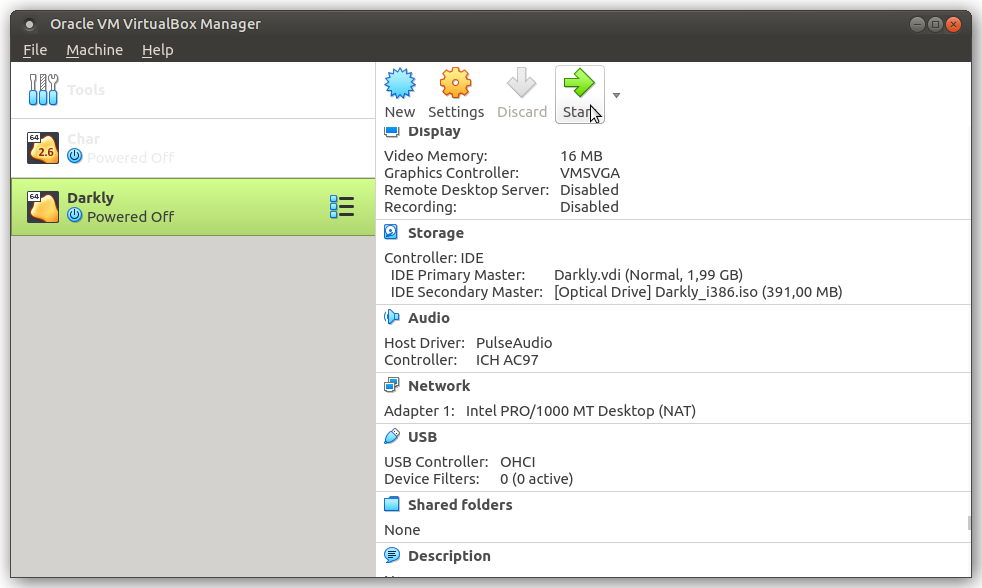
\includegraphics[width=0.752\textwidth]{images/00-07.png}\\[0cm]  
    \caption[Virtual Box]{Virtual Box Setup of Disk Drive Mount Darkly.iso Image}
    \label{fig:00-07 - Linux Virtual Box ISO Mount} 
\end{figure}
The next step is to mount the Darkly.iso disk as a form of storage. Click on
your image 'Darkly' or whatever you may have named it, on the lefthand navigation
panel as shown in Figure \Vref{fig:00-07 - Linux Virtual Box ISO Mount}.\\

Next click on Settings -> Storage -> IDE Secondary Master. After this, navigate
to the folder where the ISO is located. Mount it and you will see it listed
as shown in Figure \Vref{fig:00-07 - Linux Virtual Box ISO Mount}.\\

Click Start (Green arrow pointing right) to commence running the image.

%---------------------
\subsubsection{Run Disk Image}
\begin{figure}[!htb]
    \centering
    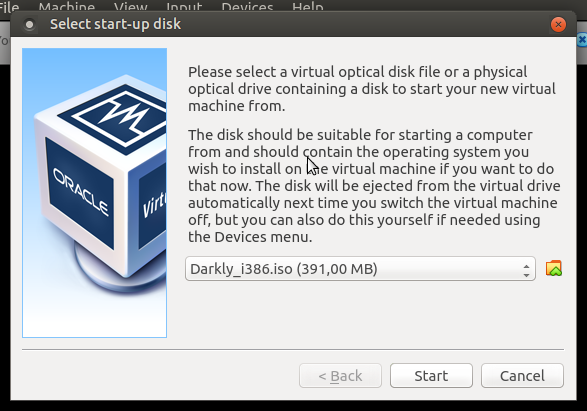
\includegraphics[width=0.752\textwidth]{images/00-08.png}\\[0cm]  
    \caption[Virtual Box]{Virtual Box Start-up Disk Selector}
    \label{fig:00-08 - Linux Virtual Box Startup Disk Selector} 
\end{figure}
As shown in Figure ~\vref{fig:00-08 - Linux Virtual Box Startup Disk Selector},
you are expected to select 'Darkly\_i386.iso' as the start-up disk. This will
then complete the Installation process.

%---------------------
\subsubsection{Running but Incomplete}
\begin{figure}[!htb]
    \centering
    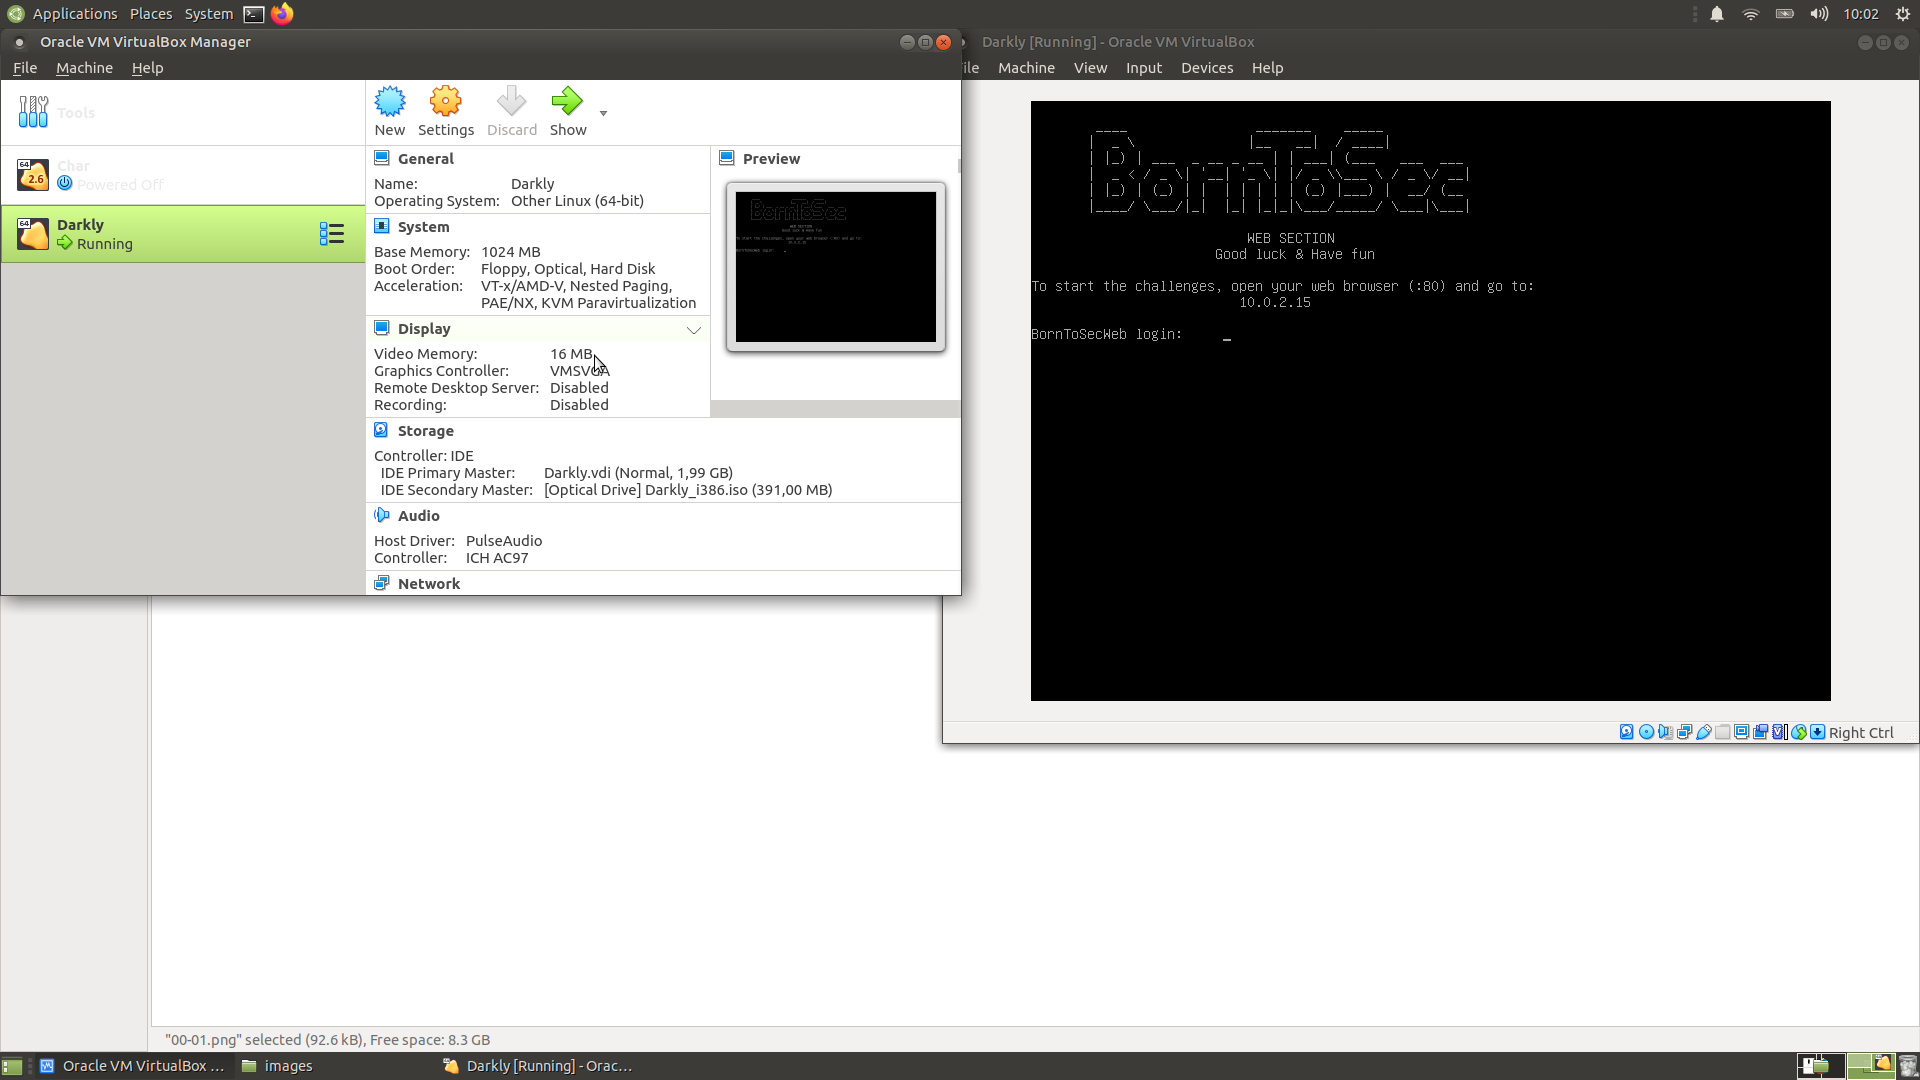
\includegraphics[width=0.752\textwidth]{images/00-09.png}\\[0cm]  
    \caption[Virtual Box]{\emph{Virtual Box Landing}, on Ubuntu}
    \label{fig:00-09 - Linux Virtual Box Running not complete} 
\end{figure}
You have successfully installed the VM and it is running. The IP address is
printed on the screen. ...I bet that the IP address does not really work\dots\\

This needs you to go to settings as shown in Figure \vref{fig:00-10 - Linux Virtual Box Set Bridge}

%---------------------
\subsubsection{Set Network Bridge}

\begin{figure}[!htb]
    \centering
    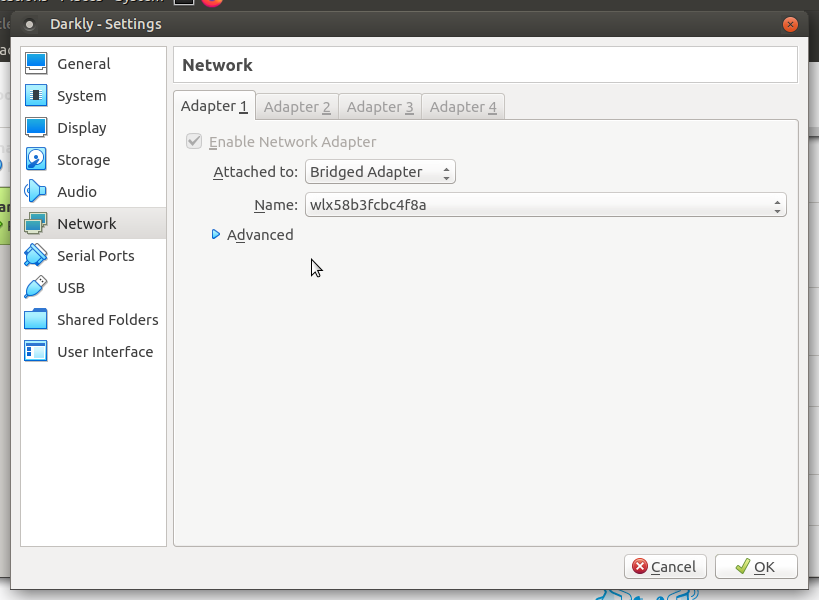
\includegraphics[width=0.752\textwidth]{images/00-10.png}\\[0cm]  
    \caption[Virtual Box]{Set the Network to Bridge not NAT}
    \label{fig:00-10 - Linux Virtual Box Set Bridge} 
\end{figure}
On the lefthand navigation-bar, Select Network -> Adaptor 1.
Change the settings from a NAT Adaptor as would be the default, and set it
to a 'Bridge' connection. as shown in Figure \vref{fig:00-10 - Linux Virtual Box Set Bridge}.

%---------------------
\subsubsection{Don't Panic! Loading Screen}

\begin{figure}[!htb]
    \centering
    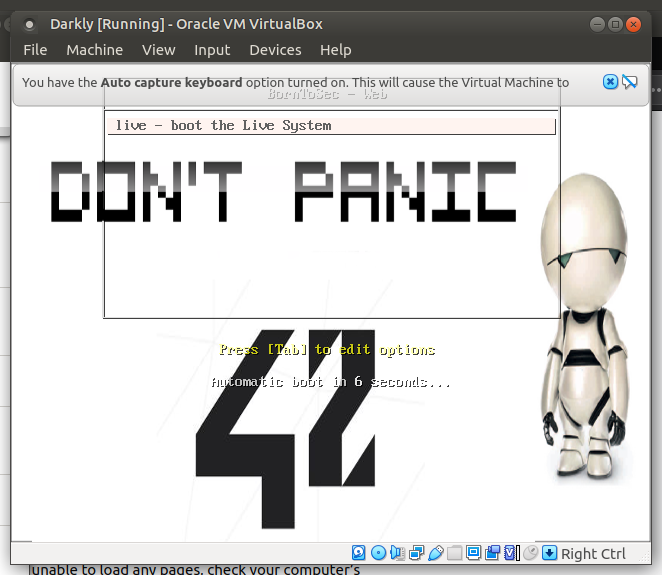
\includegraphics[width=0.752\textwidth]{images/00-11.png}\\[0cm]  
    \caption[Virtual Box]{Virtual Box Loading Screen Splash with Hitchhiker's Guide Robot}
    \label{fig:00-11 - Linux Virtual Box LoadingScreen1} 
\end{figure}
\subparagraph{Don't Panic, it's just a loading screen}

%---------------------
\subsubsection{More Loading Screens}
\begin{figure}[!htb]
    \centering
    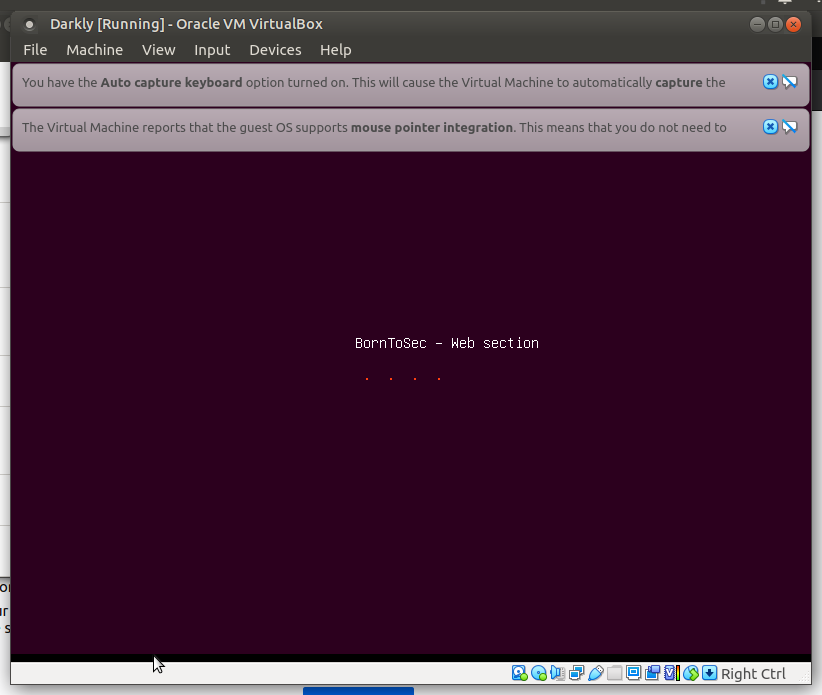
\includegraphics[width=0.752\textwidth]{images/00-12.png}\\[0cm]  
    \caption[Virtual Box]{More Virtual Box Loading Screens}
    \label{fig:00-12 - Linux Virtual Box LoadingScreen2} 
\end{figure}
If you are seeing the figure shown in Figure \vref{fig:00-12 - Linux Virtual Box LoadingScreen2}
you are making good progress and must hang in there.

%---------------------
\subsubsection{Up \& Running}

\begin{figure}[!htb]
    \centering
    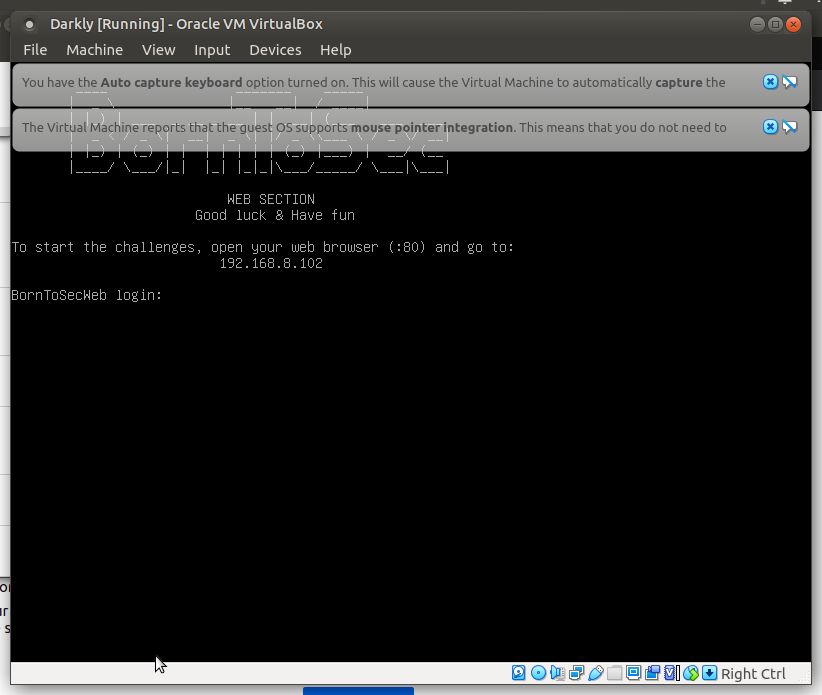
\includegraphics[width=0.752\textwidth]{images/00-13.png}\\[0cm]  
    \caption[Virtual Box]{Virtual Box Fully Loaded Screen with IP Address \& Prompt}
    \label{fig:00-13 - Linux Virtual Box LoadedIP} 

\end{figure}
The new IP Address should look different to the first one and should be similar to
your own IP address after runnung 'ifconfig'.
You should see a similar figure to that shown in Figure \vref{fig:00-13 - Linux Virtual Box LoadedIP}.

%---------------------
\subsubsection{BornToSec}
\begin{figure}[!htb]
    \centering
    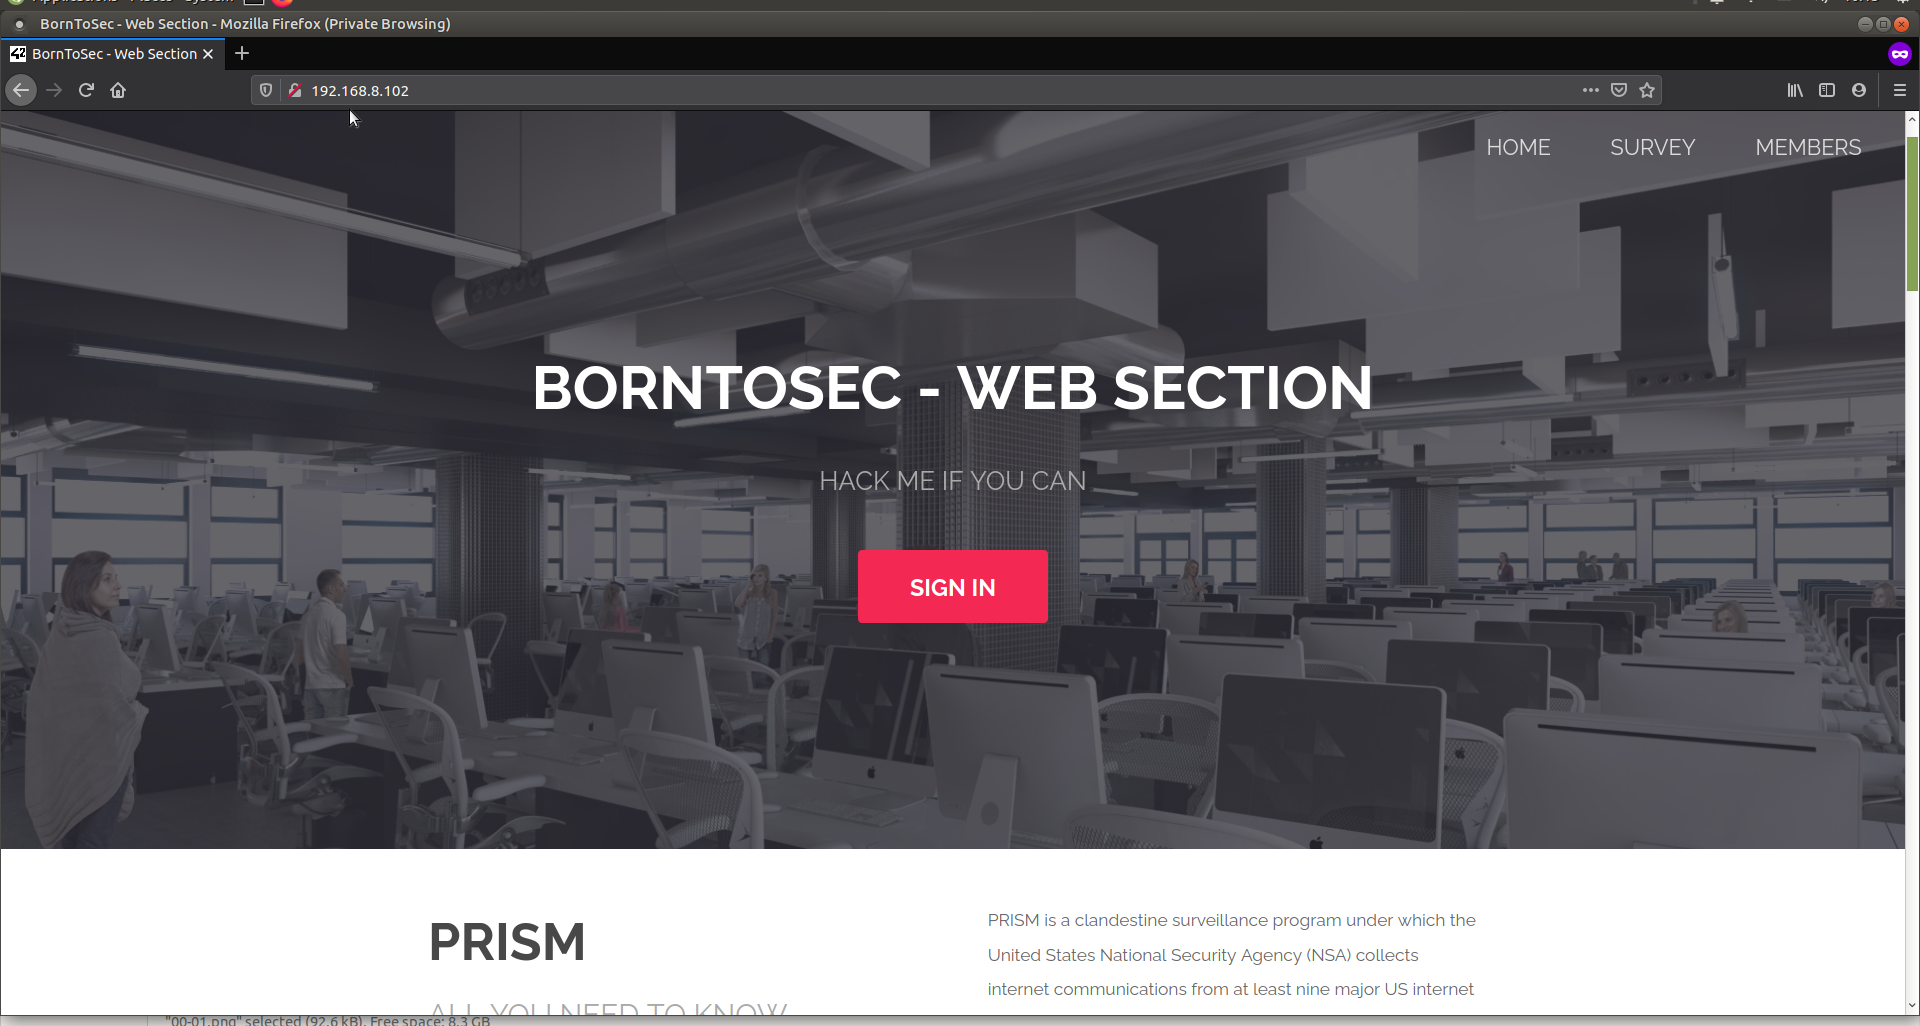
\includegraphics[width=0.752\textwidth]{images/00-14.png}\\[0cm]  
    \caption[Virtual Box]{BornToSec Homepage}
    \label{fig:00-14 - Linux Virtual Box HomePage} 
\end{figure}
If you see the same figure on your screen as the one shown on Figure \vref{fig:00-14 - Linux Virtual Box HomePage},
then you have successfully setup your Virtual Machine.

\paragraph{Time To DO The FUN Stuff!}

\clearpage


\subsection{MacOS}
At the time of typing this document a Mac was not available to conduct testing
but the documentation\cite{Docker:Mac_Install} does have instructions

\clearpage


%\vfill

%----------------------------------------------------------------------------------------

%\newpage % Start the article content on the second page, remove this if you have a longer abstract that goes onto the second page
%----------------------------------------------------------------------------------------
%	Flag \#00
%----------------------------------------------------------------------------------------

\section{Flag 00 - SQL Injection (Basic)}

\paragraph{10a16d834f9b1e4068b25c4c46fe0284e99e44dceaf08098fc83925ba6310ff5}
\begin{center}
    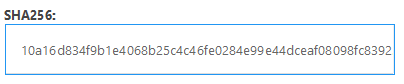
\includegraphics[width=0.5\textwidth]{03.Flag00/00-08.png}\\[0cm] 
\end{center}

The integrity of data and it's storage and retrieval is key to a successful
Web Application.

\subsection{Vulnerability}

The input bar allows a person to do raw database search with an open
'WHERE' clause for SQL Queries. This is dangerous as data remains unprotected. Countries
like South Africa have the POPI act which means that every effort must be made to keep
people's private information safe and free from a breach.

\subsection{Location}

http://<ip-address>:80/?page=member

\subsection{Method}

The way to get started is typing in an ID, it is an integer between
1 and $\infty$. You can see that ID for member 1 as shown in 
Figure~\vref{fig: 00-01 - Search start}. The next step is to try inject
your own SQL commands into the query\cite{W3Schools-SQLInjection}.

The next thing is to run '105 OR 1=1' as shown in Figure~\vref{fig: 00-02 - 105query}, the number 105 is arbitrary and can be
substituted with anything. You will see the results as shown in Figure~\vref{fig: 00-03 - 105query result}
which list everything in the database. You will notice that one of the Flags has first-name: "Flag"
Surname: "GetThe".

To see this illustrated properly just search user member '5'. This is shown in
Figure~\vref{fig: 00-04 - Get The Flag}. We have confirmation that the flag is
there.

The next step is finding the table names, run this command query
\begin{quote}
5 UNION SELECT TABLE\_NAME, COLUMN\_NAME FROM INFORMATION\_SCHEMA.COLUMNS
\end{quote}
and you will see the users, guestbook \& list\_images tables in the database. The
database that we are interested in, is the users table.

\begin{center}
    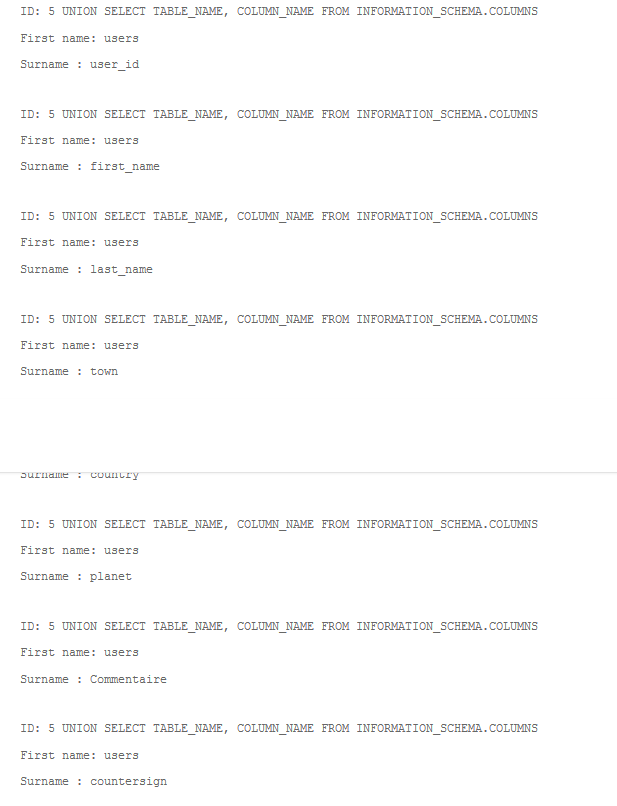
\includegraphics[width=0.5\textwidth]{03.Flag00/00-05.png}\\[0cm]    
\end{center}

You will have to run commands substituting the value of 'TABLE\_NAME' \&
COLUMN\_NAME  with the columns that you want. As shown in the
image of the query result. We are interested in only two columns in the
users table. 'Commentaire' and 'countersign' therefore we run this query
\begin{quote}
    5 UNION SELECT Commentaire, countersign FROM users
\end{quote}

\subsection{Tools}

\begin{figure}[!htb]
    \centering
    \subfloat[Search ID Member 1]{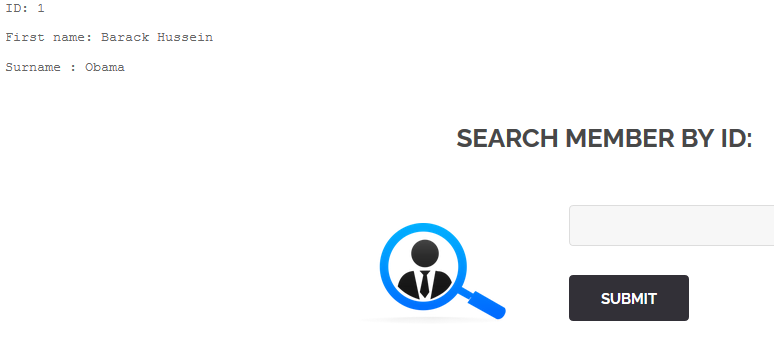
\includegraphics[width=.45\columnwidth]{03.Flag00/00-03.png}\label{fig: 00-01 - Search start}} \quad
    \subfloat[105 OR 1=1]{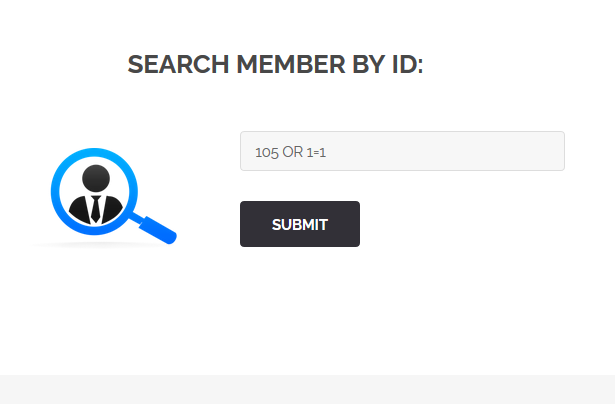
\includegraphics[width=.45\columnwidth]{03.Flag00/00-01.png}\label{fig: 00-02 - 105query}} \\
    \subfloat[Results of query]{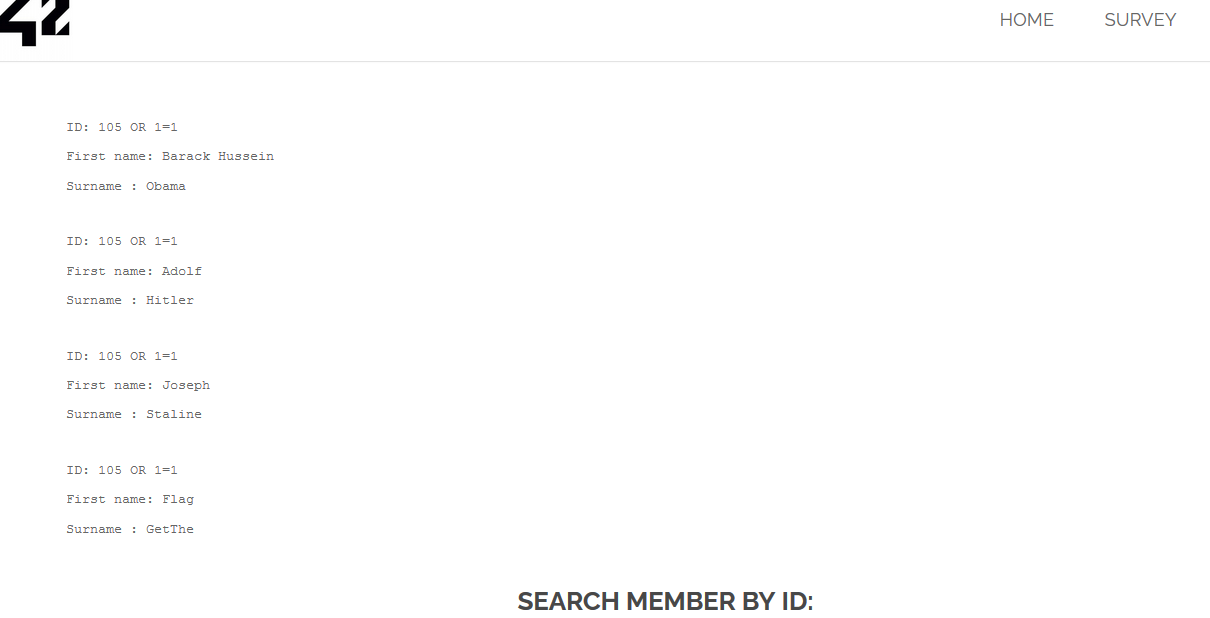
\includegraphics[width=.45\columnwidth]{03.Flag00/00-02.png}\label{fig: 00-03 - 105query result}} \quad
    \subfloat[Flag at Member Id: 5]{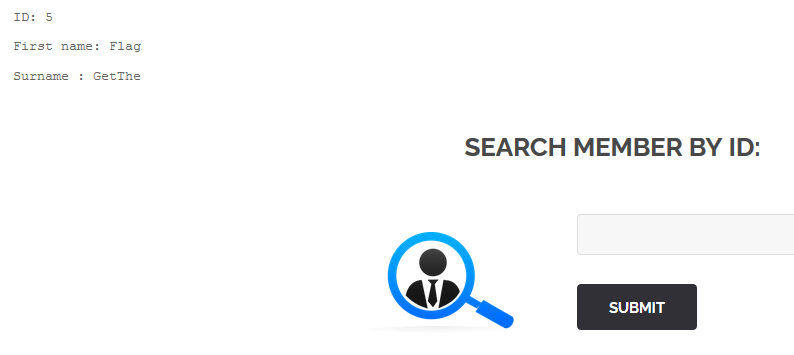
\includegraphics[width=.45\columnwidth]{03.Flag00/00-04.png}\label{fig: 00-04 - Get The Flag}}
    \caption[Flag 00 Method]{Process to Capture the SQL (Basic) Flag} % The text in the square bracket is the caption for the list of figures while the text in the curly brackets is the figure caption
    \label{fig:flag00 method}
\end{figure}
The tools used were \href{https://hashes.com/en}{hashes.com} and \href{https://www.owasp.org/index.php/SQL\_Injection}{OWASP} inlcuding
but not limited to the references cited in the Bibliography.

\subsection{Remedy}

Prepared Statements
Sanitise
\clearpage

%----------------------------------------------------------------------------------------
%	Flag \#01
%----------------------------------------------------------------------------------------

SQL Injection Advanced
\clearpage

%----------------------------------------------------------------------------------------
%	Flag \#02
%----------------------------------------------------------------------------------------

\section{Flag 02 - Include}

\paragraph{b12c4b2cb8094750ae121a676269aa9e2872d07c06e429d25a63196ec1c8c1d0}

\begin{center}
    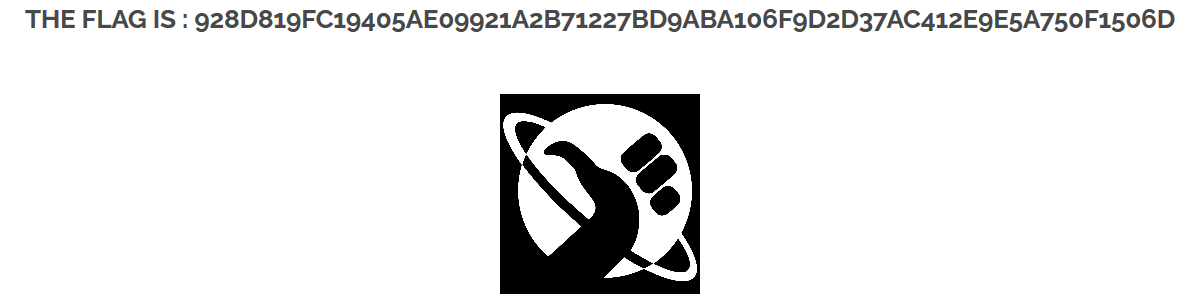
\includegraphics[width=0.5\textwidth]{05.Flag02/02-07.png}\\[0cm] 
\end{center}

\subsection{Vulnerability}

This is a classic attack often refered to as a `Directory Traversal Attack`.

\subsection{Location}

http://<ip-address>:80/index.php?page=../../../../../../../../../etc/passwd

\subsection{Method}

If you open Object Inspection Tool, you will see under the Network Tab that you are able to view the HTTP Headers. The one to look out for is `X-Powered-By PHP/5.3.10-1ubuntu3.19`.

It being `ubuntu` tells us that it is using a Unix File system. Therefore we are looking to see if we can gain access to `etc\\passwd`.

If you check the example on \href{https://en.wikipedia.org/wiki/Directory\_traversal\_attack}{Wikipedia}, the example states:

```

GET /vulnerable.php HTTP/1.0

Cookie: TEMPLATE=../../../../../../../../../etc/passwd

```

so the plan was to see if this will work if I tried to traverse the includes() until reaching the root directory.

This means consistently appending `../` until reaching the root directory.

\subsection{Tools}

\begin{figure}[!htb]
    \centering
    \subfloat[Wtf ?]{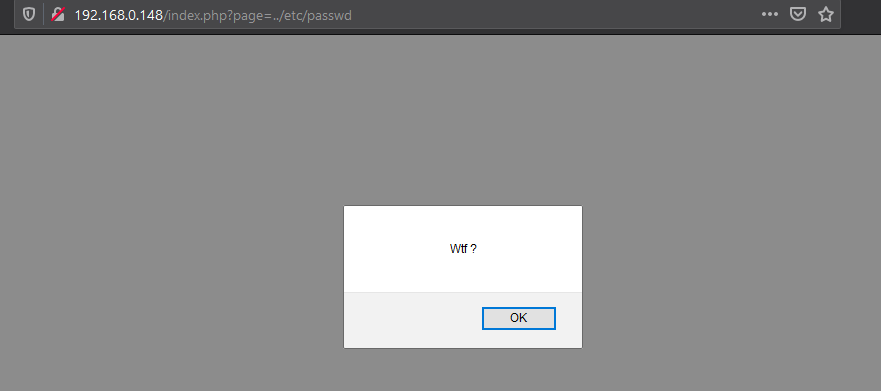
\includegraphics[width=.45\columnwidth]{05.Flag02/02-01.png}\label{fig: 02-01 - wtf}} \quad
    \subfloat[Wrong..]{
\includegraphics[width=.45\columnwidth]{05.Flag02/02-02.png}\label{fig: 02-02 - wrong}} \\
    \subfloat[Nope..]{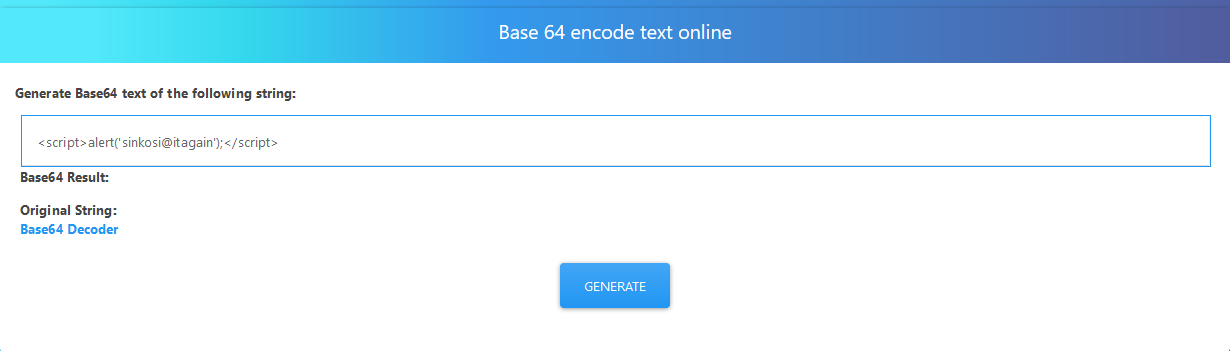
\includegraphics[width=.45\columnwidth]{05.Flag02/02-03.png}\label{fig: 02-03 - nope}} \quad
    \subfloat[Almost]{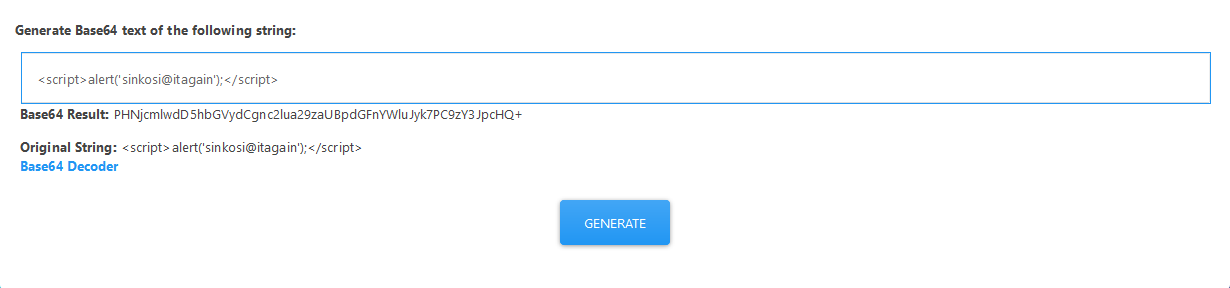
\includegraphics[width=.45\columnwidth]{05.Flag02/02-04.png}\label{fig: 02-04 - almost}}
    \subfloat[Still nope]{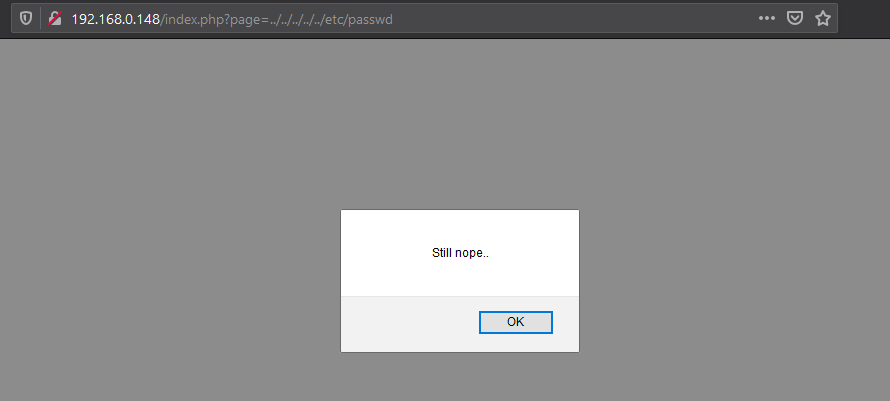
\includegraphics[width=.45\columnwidth]{05.Flag02/02-05.png}\label{fig: 02-05 - still nope}} \quad
    \subfloat[More Nope]{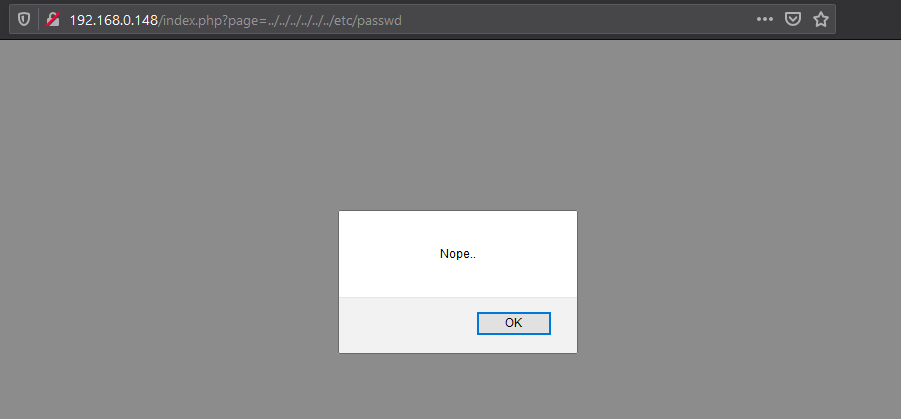
\includegraphics[width=.45\columnwidth]{05.Flag02/02-06.png}\label{fig: 02-06 - Nope..}}
    \caption[Flag 02 Method]{Process to Capture the Include Flag} % The text in the square bracket is the caption for the list of figures while the text in the curly brackets is the figure caption
    \label{fig:flag02 method}
\end{figure}

\begin{itemize}
    \item Mozilla Firefox Inspection Tool
    \item \href{https://en.wikipedia.org/wiki/Directory\_traversal\_attack}{Wikipedia - Directory Traversal Attack}
    \item \href{https://owasp.org/www-community/attacks/Path\_Traversal}{OWASP - Path Traversal}
\end{itemize}

\subsection{Remedy}

\begin{itemize}
    \item Process URI requests that do not result in a file request, e.g., executing a hook into user code, before continuing below.
    \item When a URI request for a file/directory is to be made, build a full path to the file/directory if it exists, and normalize all characters (e.g., %20 converted to spaces).
    \item It is assumed that a 'Document Root' fully qualified, normalized, path is known, and this string has a length N. Assume that no files outside this directory can be served.
    \item Ensure that the first N characters of the fully qualified path to the requested file is exactly the same as the 'Document Root'.
    
    If so, allow the file to be returned.
    If not, return an error, since the request is clearly out of bounds from what the web-server should be allowed to serve.
    
    \item Using a hard-coded predefined file extension to suffix the path does not limit the scope of the attack to files of that file extension.
    
\end{itemize}
\clearpage

%----------------------------------------------------------------------------------------
%	Flag \#03
%----------------------------------------------------------------------------------------

\section{Flag 03 - XSS Basic}

%\paragraph{df2eb4ba34ed059a1e3e89ff4dfc13445f104a1a52295214def1c4fb1693a5c3}
\begin{center}
    %\includegraphics[width=0.5\textwidth]{3.cookies/01-03.png}\\[0cm] 
\end{center}

\subsection{Vulnerability}

\subsection{Location}

\subsection{Method}

\subsection{Tools}

\subsection{Remedy}
\clearpage

%----------------------------------------------------------------------------------------
%	Flag \#04
%----------------------------------------------------------------------------------------

\section{Flag 04 - Cookies}

\paragraph{df2eb4ba34ed059a1e3e89ff4dfc13445f104a1a52295214def1c4fb1693a5c3}
\begin{center}
    \includegraphics[width=0.5\textwidth]{07.Flag04/01-03.png}\\[0cm] 
\end{center}

It's possible for an attacker to steal and reuse
session identifiers or other sensitive cookie values
when they are stored or transmitted insecurely\cite{OWASPCookie}.

\subsection{Vulnerability}

\begin{figure}[!htb]
    \centering
    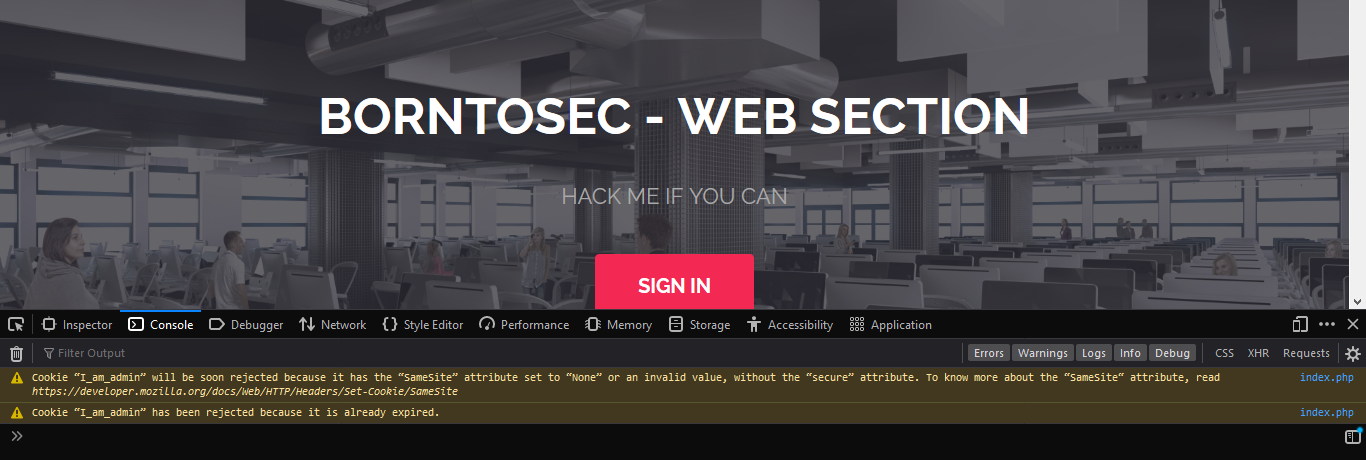
\includegraphics[width=0.752\textwidth]{07.Flag04/01-01.png}\\[0cm]  
    \caption[Cookie Alert]{Firefox refusing to set cookie `I\_am\_admin'}
    \label{fig:03-01 - Firefox rejects cookie iamadmin} 
\end{figure}
A cookie Vulnerability which is identified by OWASP as a
method to 'session-jack'\cite{OWASPCookie}.

\subsection{Location}

<ip-address>:80/index.php but also throughout the Web Application.

\subsection{Method}

I was immediately alerted by my console, for inspecting elements on
a webpage that there was something wrong with the cookie.

I proceeded to check the contents of the cookie and it was
an arbitrary string '68934a3e9455fa72420237eb05902327' (Figure \vref{fig: 3-2a cookie string}). The
cookie in question had:
\begin{itemize}
    \item[SameSite] - None
    \item[HttpOnly] - false
    \item[Secure] - false
\end{itemize}
It becomes clear what was to happen next which is determine if the string
has any meaning. After working out that the hash translated to 'false', I
decided to hash my own string equal to the string 'true'.
After refreshing the browser, the flag was returned.

The string 'true' = b326b5062b2f0e69046810717534cb09

\subsection{Tools}

\begin{figure}[!htb]
    \centering
    \subfloat[Console Screen showing cookie error]{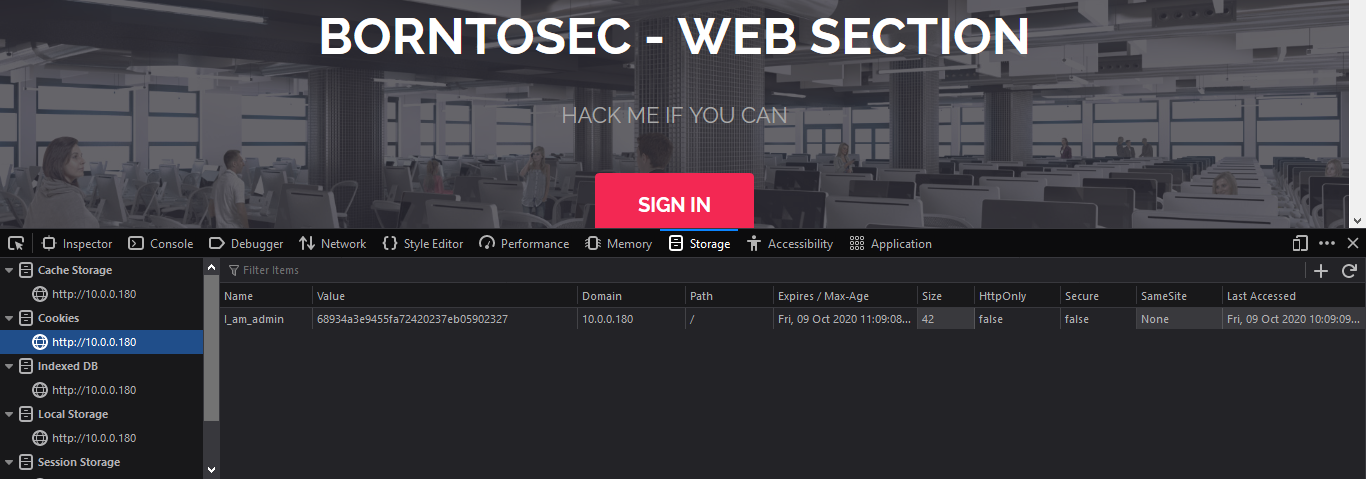
\includegraphics[width=.45\columnwidth]{07.Flag04/01-02a.png}\label{fig: 3-2a cookie string}} \quad
    \subfloat[Hash returning 'false']{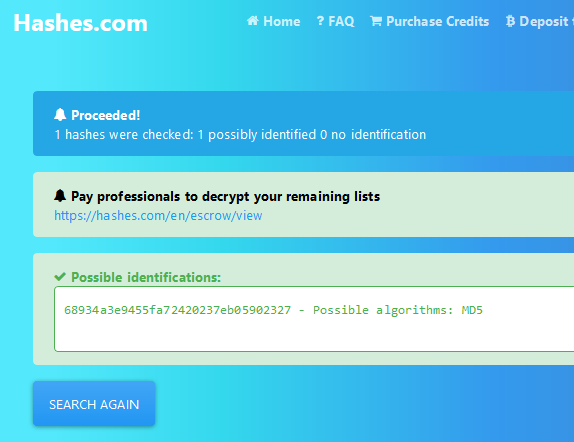
\includegraphics[width=.45\columnwidth]{07.Flag04/01-02b.png}\label{fig: cookie hash is false}} \\
    \subfloat[My own 'true' hash]{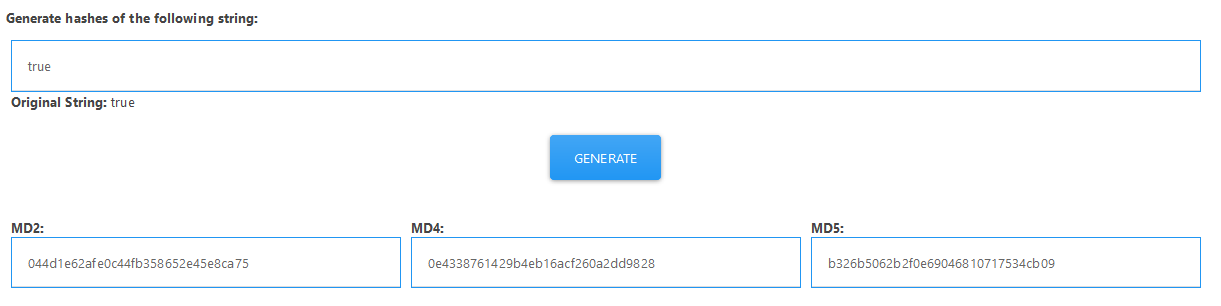
\includegraphics[width=.45\columnwidth]{07.Flag04/01-02c.png}\label{fig: 01 - My own true hash}} \quad
    \subfloat[Replaced hash \& ready to refresh]{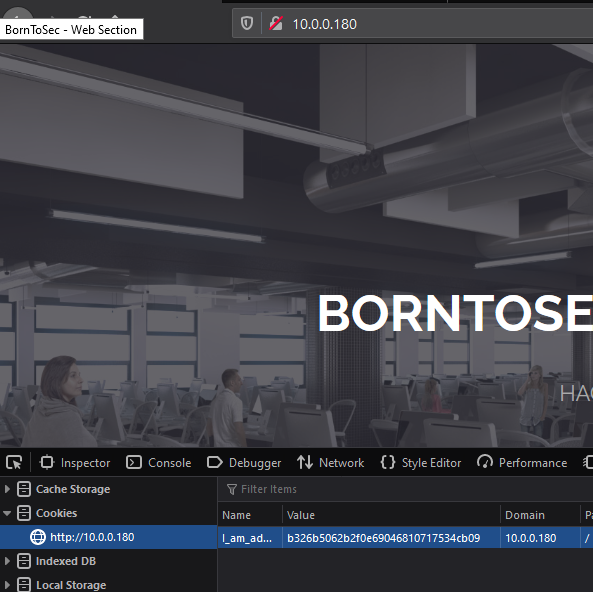
\includegraphics[width=.45\columnwidth]{07.Flag04/01-02d.png}\label{fig: 01 - Ready to refresh}}
    \caption[Flag 01 Method]{Process to Capture the Cookie Flag} % The text in the square bracket is the caption for the list of figures while the text in the curly brackets is the figure caption
    \label{fig:flag1 collection}
\end{figure}

The tools that I used were the console output of the 'Inspection Tool'
and the website \href{http://www.hashes.com}{hashes.com} in order to work
with the hashes.

\subsection{Remedy}

According to OWASP\cite{OWASPCookie} these are the steps one can take:
\begin{itemize}
    \item Make sure that all session identifiers are transmitted over an encrypted protocol.
    \item Terminate/regenerate the session if the session token is transmitted insecurely (either in clear text or as part of the URL), or signal to the application to do so.
    \item Enforce the Secure and HttpOnly flags on sensitive cookies using a Web Application Firewall.
    \item Ensure that session identifiers are transmitted only using the SSL session where they originated. Track sessions across SSL renegotiations and integrate with framework solutions to support common SSL termination/re-encryption architectures.
\end{itemize}
\clearpage

%----------------------------------------------------------------------------------------
%	Flag \#05
%----------------------------------------------------------------------------------------

\section{Flag 05 - Spoof (Curl)}

%\paragraph{df2eb4ba34ed059a1e3e89ff4dfc13445f104a1a52295214def1c4fb1693a5c3}
\begin{center}
    %\includegraphics[width=0.5\textwidth]{3.cookies/01-03.png}\\[0cm] 
\end{center}

\subsection{Vulnerability}

\subsection{Location}

\subsection{Method}

\subsection{Tools}

\subsection{Remedy}
\clearpage

%----------------------------------------------------------------------------------------
%	Flag \#06
%----------------------------------------------------------------------------------------

Directories

\clearpage

%----------------------------------------------------------------------------------------
%	Flag \#07
%----------------------------------------------------------------------------------------

\section{Flag 07 - Bruteforce (member)}

\paragraph{b3a6e43ddf8b4bbb4125e5e7d23040433827759d4de1c04ea63907479a80a6b2}
\begin{center}
    \includegraphics[width=0.5\textwidth]{10.Flag07/07-04.png}\\[0cm] 
\end{center}

\subsection{Vulnerability}

Brute-force attacks are often used for attacking authentication and discovering hidden content/pages within a web application. These attacks are usually sent via GET and POST requests to the server. In regards to authentication, brute force attacks are often mounted when an account lockout policy is not in place.

\subsection{Location}

'http://<ip-address>:80/?page=signin'

\subsection{Method}

When one opens that `<ip-address>`, you are greeted by a `SIGN IN` button. When you click on it, you will notice a login page with the Bot from that one movie/book.

You wish to gain elevated priviledges so you will want to try log in as an admin. You will see when you analyse the code that the form uses a GET method and names its two inputs as username \& password respectively:


```

<td style="vertical-align:middle;">
  
    <form action="\#" method="GET">

    <input type="hidden" name="page" value="signin">
    
    Username:<input type="text" name ="username" style="width:100%;">

</td>

</tr>

<tr style="background-color:transparent;border:none;">
  
    <td style="vertical-align:middle;">
    
        Password:<input type="password" name ="password" style="width:100%;" AUTOCOMPLETE="off">
        
    </td>

</tr>

```

So the plan is to `spam` the URL over and over until the correct password is accepted. This is done via trying a list of passwords and seeing which one is eventually accepted. Here is the code:

```

for i in \${password[@]}; do
    
    if curl --silent -X POST "http://\${ip}/index.php?page=signin\&username=admin\&password=\${i}\&Login=Login\#" | grep "flag";
    
    then
    
        echo -e "\\nPassword is: \$i"
        
        curl -o sinkosi.html -X POST "http://\${ip}/index.php?page=signin\&username=admin\&password=\${i}\&Login=Login\#"
        
        exit 1
    
    fi

done

echo -e "\\nPassword is not in list\\n"

```

When the password is successfully found it will be printed to the terminal and a file sinkosi.html will be created. Open the html file, and the flag will be there.

*Alternative:* Use the retrieved password printed on the terminal and login directly on the VM.

\subsection{Tools}

\begin{figure}[!htb]
    \centering
    \subfloat[Sign In Link]{\includegraphics[width=.45\columnwidth]{10.Flag07/07-01.png}\label{fig: 07-01 - wtf}} \quad
    \subfloat[Credentials Requested]{\includegraphics[width=.45\columnwidth]{10.Flag07/07-02.png}\label{fig: 07-02 - wrong}} \\
    \subfloat[Credentials entered]{\includegraphics[width=.45\columnwidth]{10.Flag07/07-03.png}\label{fig: 07-03 - nope}} \quad
    \subfloat[Retrieved Flag]{\includegraphics[width=.45\columnwidth]{10.Flag07/07-04.png}\label{fig: 07-04 - wrong}} \\
    \caption[Flag 07 Method]{Process to Capture the Bruteforce Flag} % The text in the square bracket is the caption for the list of figures while the text in the curly brackets is the figure caption
    \label{fig:flag07 method}
\end{figure}

\begin{itemize}
    \item \href{https://en.wikipedia.org/wiki/List_of_the_most_common_passwords}{Wikipedia - Most Common Passwords}
    \item \href{http://securitypadawan.blogspot.com/2012/04/using-curl-to-brute-force-http-login.html}{Security Padawan}
    \item \href{https://www.comparitech.com/blog/information-security/brute-force-attack/}{CompariTech}
    
\end{itemize}

\subsection{Remedy}
Two Steps

\paragraph{How To Detect Brute Force Attack}

\begin{itemize}
    \item Multiple failed login attempts from the same IP address. Although, this could be a result of a proxy server being used by a large organization.
    \item Login attempts with multiple usernames from the same IP address. Again, this could simply be from a large organization.
    \item Multiple login attempts for a single username coming from different IP addresses. This could also be a single person using a proxy.
    \item An unusual pattern of failed login attempts, for example, following a sequential alphabetical or numerical pattern.
    \item An abnormal amount of bandwidth being used after a successful login attempt. This could signal an attack designed to steal resources.
\end{itemize} 

\paragraph{How To Prevent Brute Force Attack}
    
\begin{itemize}
    \item Utilizing or requiring strong passwords
    \item Allowing a limited number of login attempts
    \item Employing the use of CAPTCHAs
    \item Setting time delays between attempts
    \item Asking security questions
    \item Enabling or requiring two-factor authentication
    \item Using multiple login URLs
    \item Tricking the attack software (fake login)
\end{itemize}


%----------------------------------------------------------------------------------------
%	Flag \#08
%----------------------------------------------------------------------------------------

\section{Flag 08 - File Upload}

%\paragraph{df2eb4ba34ed059a1e3e89ff4dfc13445f104a1a52295214def1c4fb1693a5c3}
\begin{center}
    %\includegraphics[width=0.5\textwidth]{3.cookies/01-03.png}\\[0cm] 
\end{center}

\subsection{Vulnerability}

\subsection{Location}

\subsection{Method}

\subsection{Tools}

\subsection{Remedy}

%----------------------------------------------------------------------------------------
%	Flag \#09
%----------------------------------------------------------------------------------------

\section{Flag 09 - Redirect}

%\paragraph{df2eb4ba34ed059a1e3e89ff4dfc13445f104a1a52295214def1c4fb1693a5c3}
\begin{center}
    %\includegraphics[width=0.5\textwidth]{3.cookies/01-03.png}\\[0cm] 
\end{center}

\subsection{Vulnerability}

\subsection{Location}

\subsection{Method}

\subsection{Tools}

\subsection{Remedy}

%----------------------------------------------------------------------------------------
%	Flag \#10
%----------------------------------------------------------------------------------------

\subsection{Flag \#}

\subsubsection{Vulnerability}

\subsubsection{Location}

\subsubsection{Method}

\subsubsection{Tools}

\subsubsection{Remedy}

%----------------------------------------------------------------------------------------
%	Flag \#11
%----------------------------------------------------------------------------------------

\section{Flag 11 - Survey}

%\paragraph{df2eb4ba34ed059a1e3e89ff4dfc13445f104a1a52295214def1c4fb1693a5c3}
\begin{center}
    %\includegraphics[width=0.5\textwidth]{3.cookies/01-03.png}\\[0cm] 
\end{center}

\subsection{Vulnerability}

\subsection{Location}

\subsection{Method}

\subsection{Tools}

\subsection{Remedy}

%----------------------------------------------------------------------------------------
%	Flag \#12
%----------------------------------------------------------------------------------------

\section{Flag 12 - Recover}

%\paragraph{df2eb4ba34ed059a1e3e89ff4dfc13445f104a1a52295214def1c4fb1693a5c3}
\begin{center}
    %\includegraphics[width=0.5\textwidth]{3.cookies/01-03.png}\\[0cm] 
\end{center}

\subsection{Vulnerability}

\subsection{Location}

\subsection{Method}

\subsection{Tools}

\subsection{Remedy}

%----------------------------------------------------------------------------------------
%	Flag \#13
%----------------------------------------------------------------------------------------

\subsection{Flag \#}

\subsubsection{Vulnerability}

\subsubsection{Location}

\subsubsection{Method}

\subsubsection{Tools}

\subsubsection{Remedy}

%----------------------------------------------------------------------------------------
%	BIBLIOGRAPHY
%----------------------------------------------------------------------------------------
\section{Bibliography}

\renewcommand{\refname}{\spacedlowsmallcaps{References}} % For modifying the bibliography heading

\bibliographystyle{unsrt}

\bibliography{00.Extras/sample.bib} % The file containing the bibliography
%\bibliography{sample2.bib}

%----------------------------------------------------------------------------------------

%\end{document}


\section{Student Honesty Declaration}

Engaging in any cheating or dishonesty in any form of assessment, 
assignment, test orexamination or other WeThinkCode\_ prescribed work 
is considered cheating and is grounds for disciplinary action.
Plagiarism, which is to present work (or a portion of work) as your 
own when it is not, isconsidered cheating and is not accepted at 
WeThinkCode\_.

An evaluator can flag one for plagiarism on one of the following grounds\
:\begin{itemize}
     
\item The evaluator (marker) identifies that the student does not understand
all or part of the work they have submitted.
\item If all or part of the work presented is plagiarised ,i.e. copied from 
another source without reference.
\end{itemize}

\begin{large}\textbf{Cheating in group projects}\end{large}\\

The main purpose for a group project is to give students the experience of working in ateam, by coming up with a solution to a problem together.
\begin{itemize}
    \item Each member must be able to show which portion of the project they worked on. 
    \item Failure to do so will result in the student being flagged for cheating which will begrounds for disciplinary action.
    \item This is to avoid single members doing the majority of the group project at the benefit of a member who is not contributing.
    \item In this way we are able to ensure fair assessment of each WTC\_ student’s competence.
\end{itemize}    
Group projects can be approached in two ways.
\begin{enumerate}
    \item Divide and conquer: This is usually preferred and advised when working on big projects. The project is divided into segments, in which each member of the group can accomplish. Once completed, the group will then integrate the segments to complete the project
    \item One for all: This method is usually preferred and advised when a group is working on a small project. The group will work on the solution together from the start of the project until the end. This will require the members to move at a pace in which everyone in the team can keep up with.
\end{enumerate}    
NOTE: At the end of each group project, each member should have a general and basic understanding of the project and the solution found. This will include running,testing and explaining the solutions of the project.

\section*{Declaration}

I hereby declare that the work submitted by me and/or my group members is:
\begin{itemize}
    \item Original (not plagiarised)
    \item References listed
    \item Honest \& in Good Faith
    \item Subject to WeThinkCode\_policies
\end{itemize}

\vspace{15mm}

% \begin{minipage}{0.4\textwidth}
%     \begin{flushleft}
%         \large
%         \line(1,0){120}\\
%         Mosima \textsc{Mamaleka} % Your name
%         \textit{WeThinkCode\_ Student}\\
%     \end{flushleft}
% \end{minipage}
% ~
% \begin{minipage}{0.4\textwidth}
%     \begin{flushright}
%         \large
%         \line(1,0){120}\\
%         Sibonelo \textsc{Nkosi} % Supervisor's name
%         \textit{WeThinkCode\_ Student}\\
%     \end{flushright}
% \end{minipage}

\begin{flushleft}
\line(1,0){120}\\
Sibonelo \textsc{Nkosi}\\ % Your name
Username: \textsc{sinkosi}\\ % Your name
{\large\textit{Developer}}
\end{flushleft}


%---------------------------------------------------------------------------------------
%\printindex

\end{document}